\section{Methods} \label{s:cs:methods}



The cluster analysis can be split into three stages: 1) the data pre-processing, 2) select the clustering model, and 3) choosing the number of clusters. The first part is covered in the following section \ref{s:cs:pre-processing}, while choosing the clustering model and its configuration is presented in \cref{s:cs:right_config}.


% pre-processing
\subsection{Pre-processing} \label{s:cs:pre-processing}

% gene filtering
The RNAseq data consists of a large number of genes ($\sim$30,000), many of which are not uniformly expressed across the samples. In this section, a gene is considered unexpressed if more than 10\% of the samples have a value less than 1.5 TPM. Filtering out genes that meet these few conditions leaves TCGA's tumour dataset with approximately 13,000 genes that are expressed in at least 90\% of the samples (approximately 370 samples). The threshold of 10\% is derived from the study by \citet{Robertson2017-mg}, where the authors removed all genes that had 'NA values more than 10\% across samples' (section \textit{Unsupervised mRNA expression clustering}). However, it is important to note that the authors of that study used RSEM data, not TPMs.

From the resultant dataset, a subset of the most variably expressed genes is selected depending on the experiment. The most variably expressed genes are identified by the highest standard deviation to median ratio, which also considers the magnitude of the expression. This approach differs from that used by \citet{Robertson2017-mg}, which selects the top 25\% of genes based solely on standard deviation without factoring in the magnitude of gene expression.


% Right config
\subsection{Clustering model configuration} \label{s:cs:right_config}

In subsequent experiments, several clustering models were evaluated using the scikit-learn library \citep{Scikit-learn_undated-ax}, as introduced in \cref{s:lit:clustering}. The models tested included \gls{KMEANS}, Ward, Agglomerative Clustering, Birch, Gaussian Mixture, and Spectral Clustering. The performance of these models was assessed using clustering metrics that do not require ground truth such as Silhouette, Calinski-Harabasz, and Davies-Bouldin, detailed in \cref{s:lit:clustering_metrics}. Other clustering methods were explored but not presented as these performed poorly, typically finding one or two groups despite various configurations.


Before applying clustering methods, \gls{PCA} is employed to reduce the dimensions of the data. This dimension reduction technique notably enhances the performance of the clustering algorithms, as evidenced by the improved metric scores for PCA-transformed data, see  \cref{fig:cs:cs_metrics}, compared to non-PCA data as shown in \cref{s:ap:non-pca} from Appendix. Specifically, the Silhouette score doubles, indicating a two-fold improvement in cluster tightness and separation. The Calinski-Harabasz score sees a threefold increase, reflecting better-defined clusters, while the Davies-Bouldin score halves, suggesting a better partition (lower is better). The number of PCA components is set to 4, marking the threshold beyond which each additional component contributes less than 1\% to the overall PCA variance\footnote{The PCA variance is a measure of the information each component captures}.

\begin{figure}[!t]
    \captionsetup[subfigure]{justification=Centering}
    \centering
    \begin{subfigure}[!t]{1.0\textwidth}
        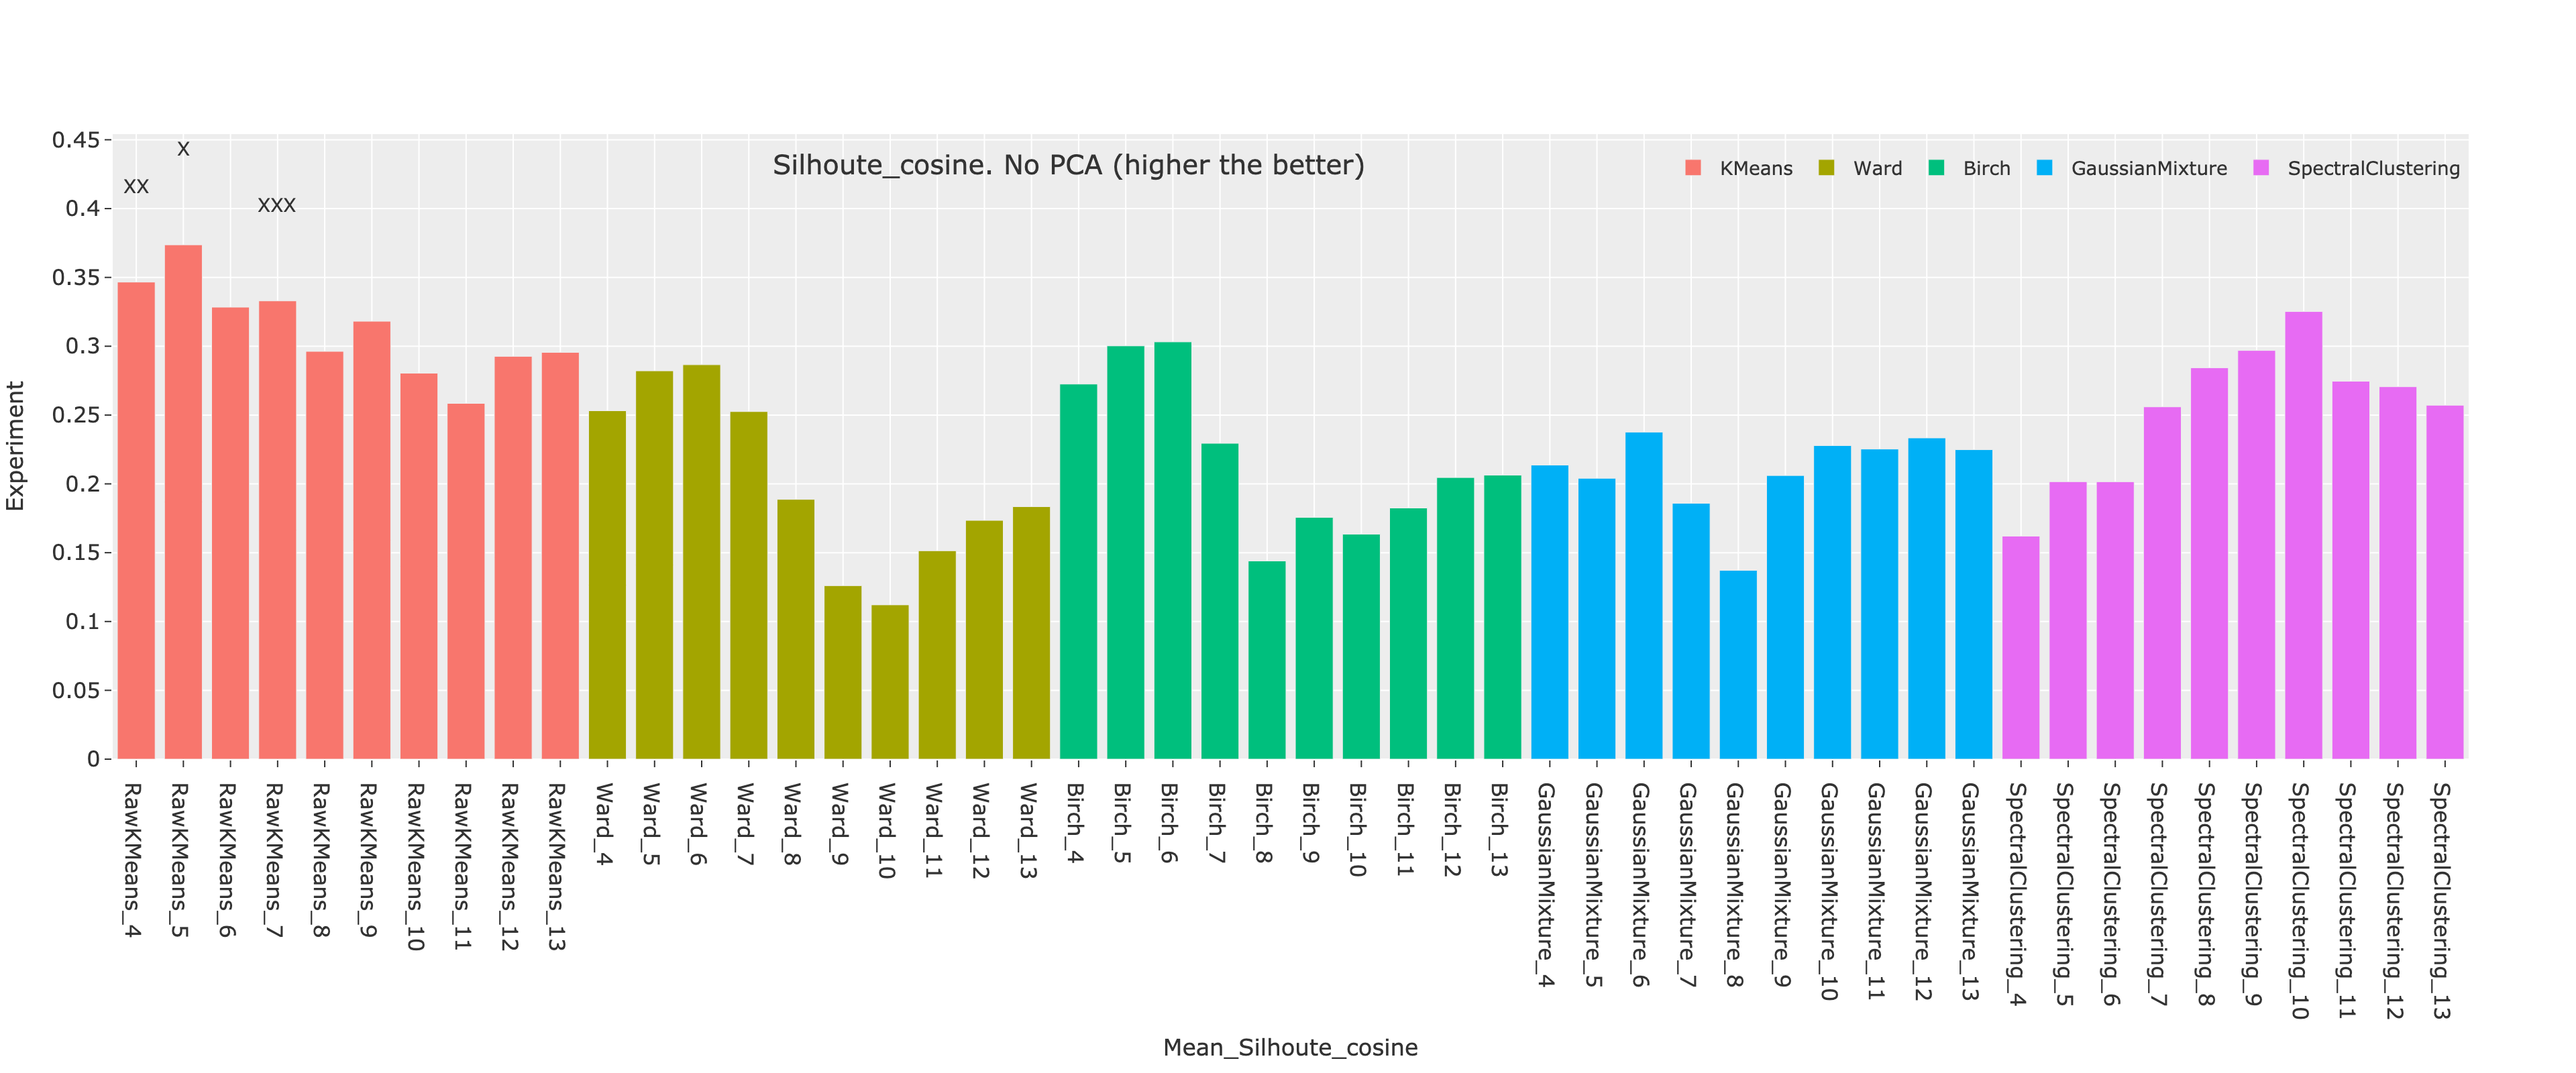
\includegraphics[width=\textwidth,keepaspectratio]{Sections/ClusteringAnalysis/Resources/cs_top3/PCA_top3_Silhoute_cosine.png}
        \caption{Silhouette using cosine distance}
        \label{fig:cs:cosine}
    \end{subfigure}
    \centering
    \begin{subfigure}[!t]{1.0\textwidth}
        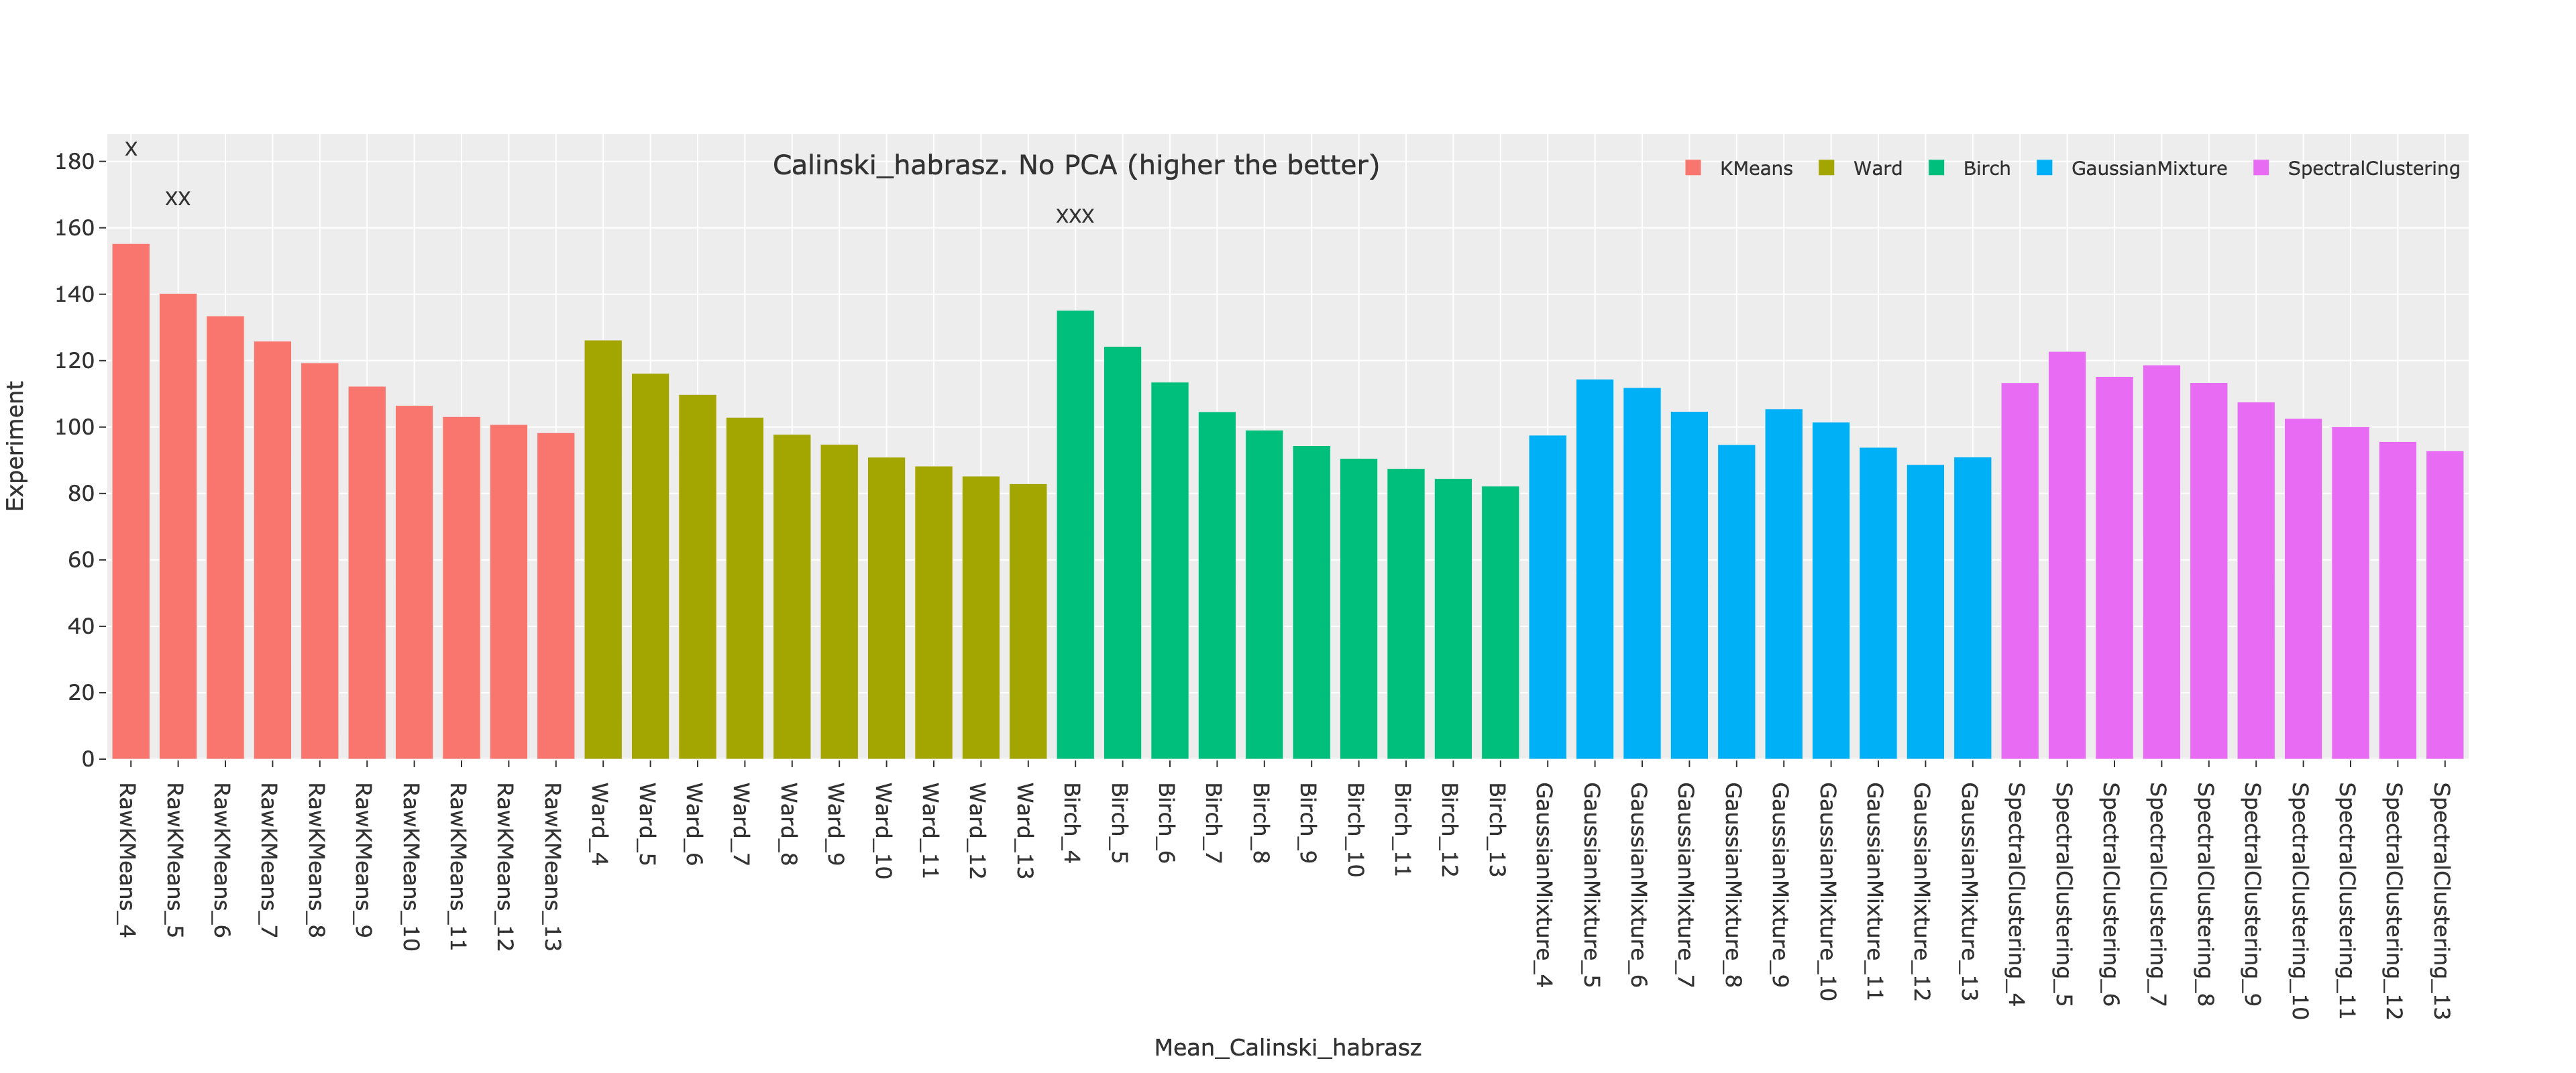
\includegraphics[width=\textwidth,keepaspectratio]{Sections/ClusteringAnalysis/Resources/cs_top3/PCA_top3_Calinski_habrasz.png}
        \caption{Calinski Harabasz}
        \label{fig:cs:cal_hab}
    \end{subfigure}
    \caption[Measuring clustering models: Silhouette and Calinski Habrasz]{The means of the two cluster metrics introduced in \cref{s:lit:clustering_metrics}: Silhouette (cosine) and Calinski Harabasz. The gene expression is processed according to \cref{s:cs:methods} and PCA with 5 components was applied. For each metric the top 3 most performing models are marked by "X". Gaussian Mixture Model is abbreviated to GM and Spectral Clustering to SC. K-means with K=4 and K=5 are the best performing clustering configuration.}
    \label{fig:cs:cs_metrics}
\end{figure}


\begin{figure}[!htb]    
    \centering
    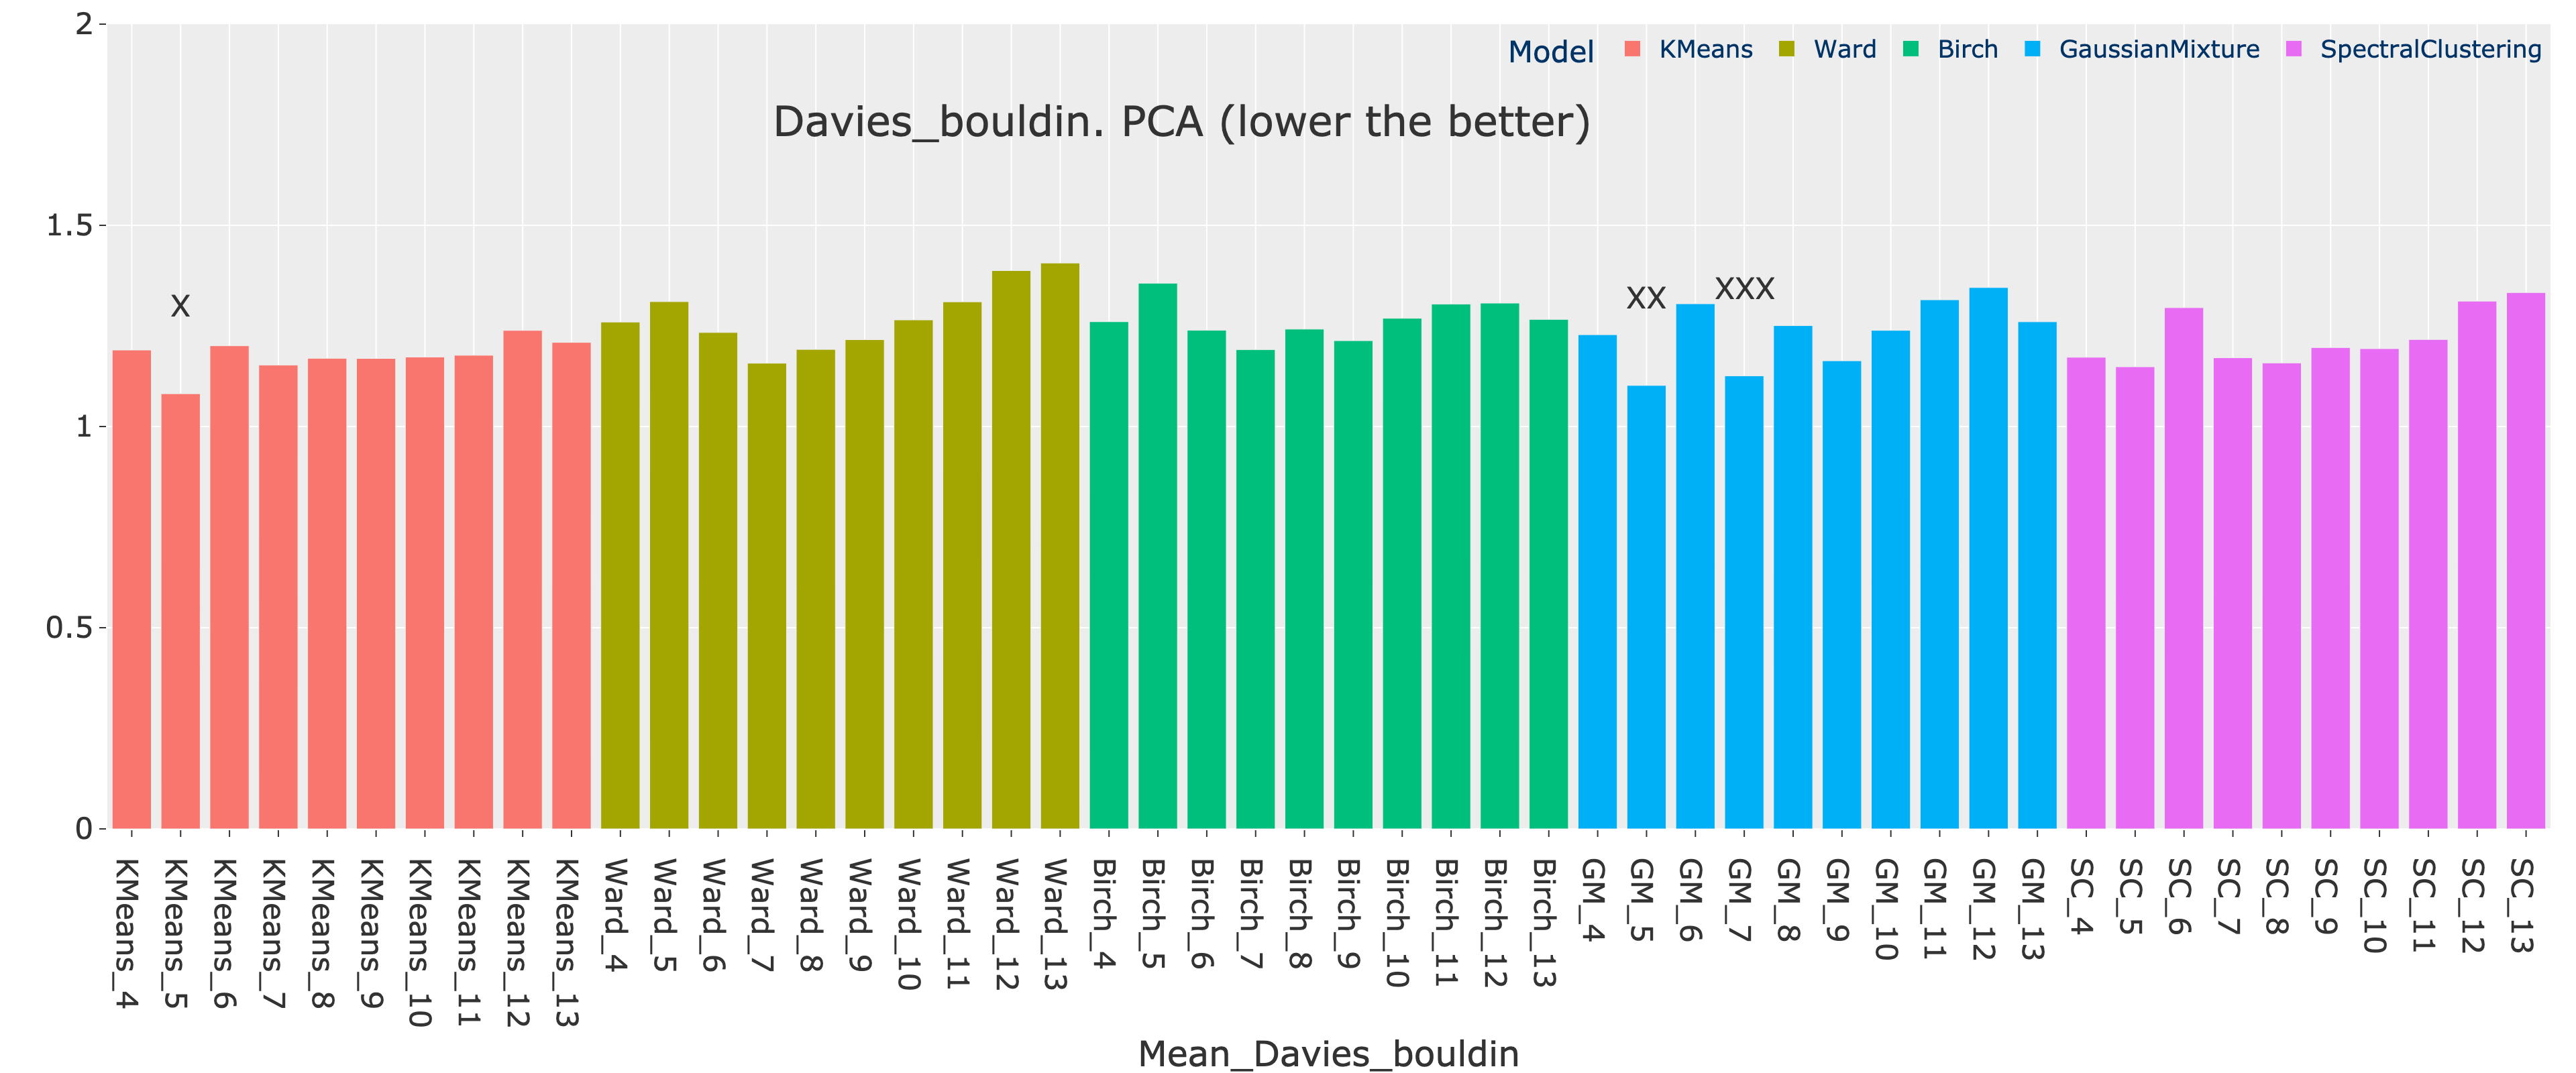
\includegraphics[width=1.0\textwidth,keepaspectratio]{Sections/ClusteringAnalysis/Resources/cs_top3/PCA_top3_Davies_bouldin.png}
    \caption[Measuring clustering models: Davies Boulding]{The means of the cluster metrics introduced in Davies Bouldin introduced in \cref{s:lit:clustering_metrics}. The gene expression is processed according to \cref{s:cs:methods} and PCA with 5 components was applied. For each metric the top 3 most performing models are marked by "X". Gaussian Mixture Model is abbreviated to GM and Spectral Clustering to SC. K-means with K=5 and Gaussian Mixture with 4 are the best two performing models.}
    \label{fig:cs:dav_boul}
\end{figure}

The performance of the five clustering methods over cluster size, K, where $K\in[4, 13]$ is displayed in \cref{fig:cs:cs_metrics,fig:cs:dav_boul}. It was empirically observed that the clustering method scored the best at $K\in\{2,3\}$, which is expected in sparse datasets. The best performing models are those with small $K$ that have little separation between the groups. The number of 'X' markers on top of the bar marks the model's position in top three. From the plots, it can be seen that K-means generally perform the best among the clustering methods. The inverse relation between the algorithm's performance over the number of groups is the most evident in the Calinski Harabasz score, in \cref{fig:cs:cal_hab} and Davies Bouldin index, see \cref{fig:cs:dav_boul}, but less pronounced in the Silhouette score as shown in \cref{fig:cs:cosine}.


To aid the decision making, the top three most performing configuration are displayed per cluster metric in \cref{fig:cs:cs_metrics_heatmap}. The two heatmaps are similar, each column represents the algorithm while the rows the cluster metrics, the colouring is done per column. The first plot indicates the most popular model configuration per algorithm, while the second the most frequent value of K. From this, K-Means with 5, Spectral Clustering with 7 clusters and K=5 and K=7 are the most frequent methods/group sizes. 

Less common in the top three best performing, are the cluster models with high number of clusters such as Wrd\_9, Birch\_11 or GaussianMixture\_8. It can also be noticed that the cluster size oscillates between 5-7 groups which is in agreement with the other classification such as TCGA (5) and consensus (6) \citep{Robertson2017-mg,Kamoun2020-tj}.

\begin{figure}[!t]
    \centering
    \small
    \begin{subfigure}[!t]{0.8\textwidth}
        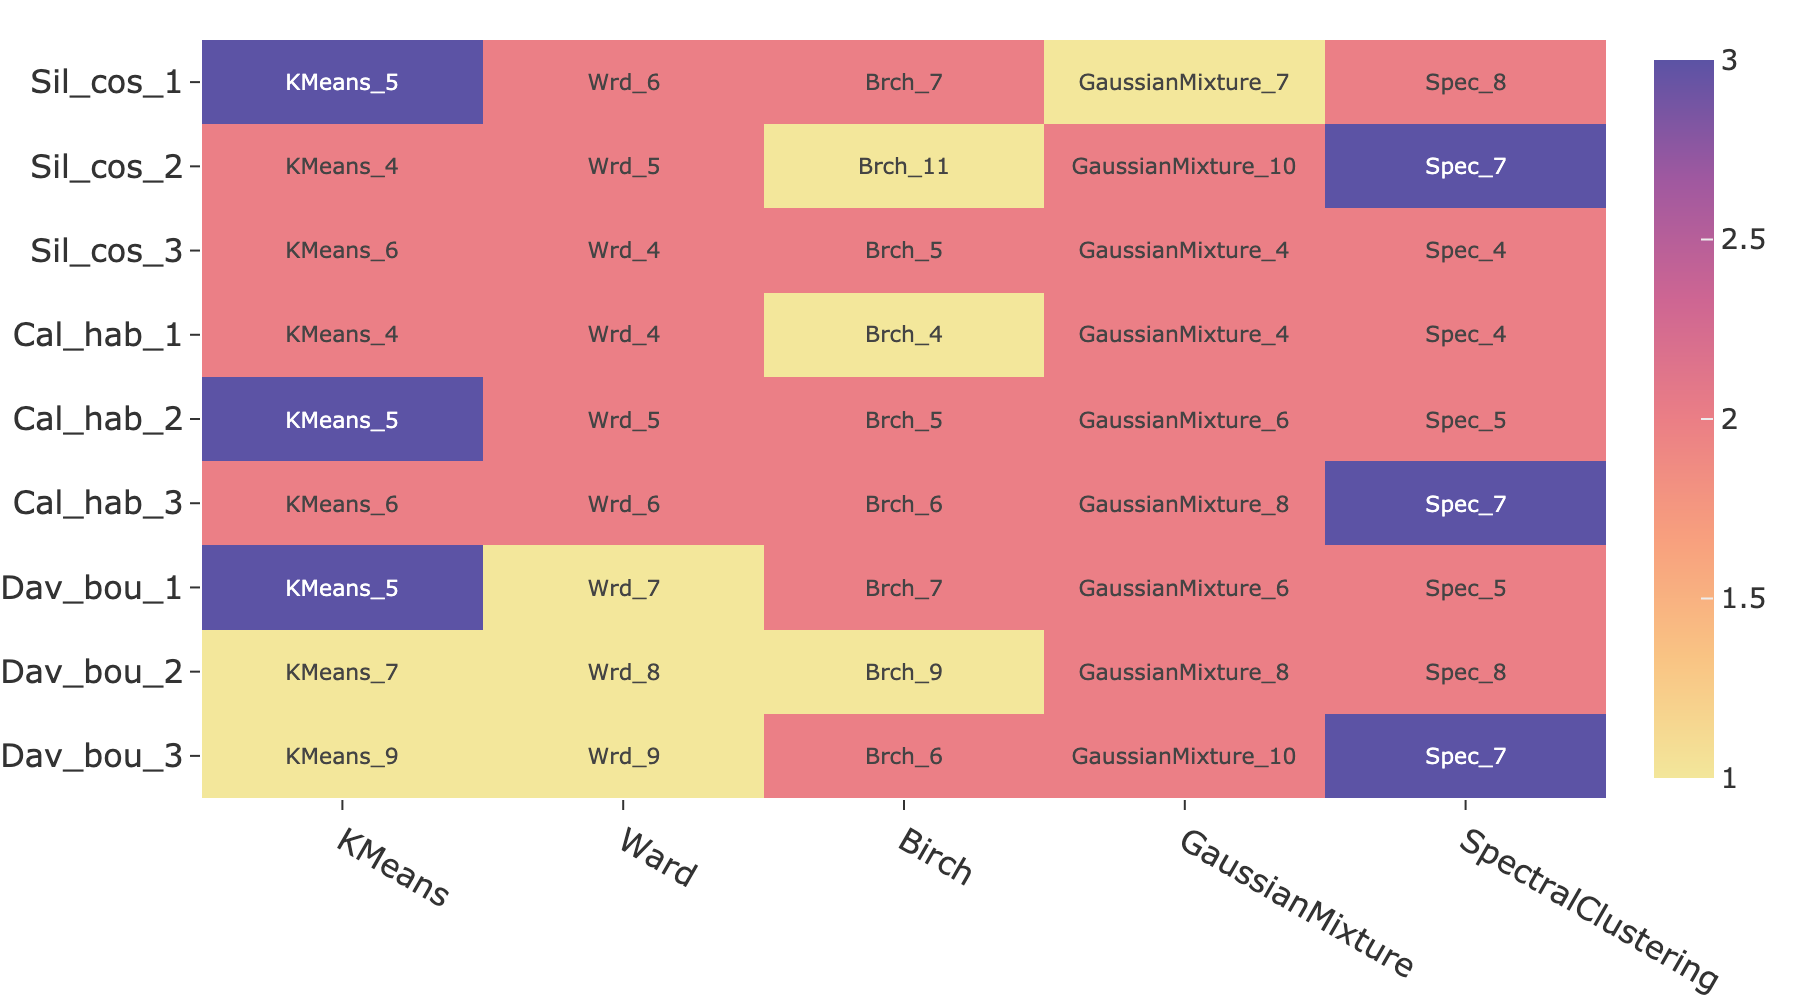
\includegraphics[width=\textwidth]{Sections/ClusteringAnalysis/Resources/cs_top3/top3_cs_gen_top3_heatmap_pca.png}
        \caption{Most frequent cluster model configuration}
        \label{fig:cs:heatmap_gen}
    \end{subfigure}
    \centering
    \begin{subfigure}[!t]{0.8\textwidth}
        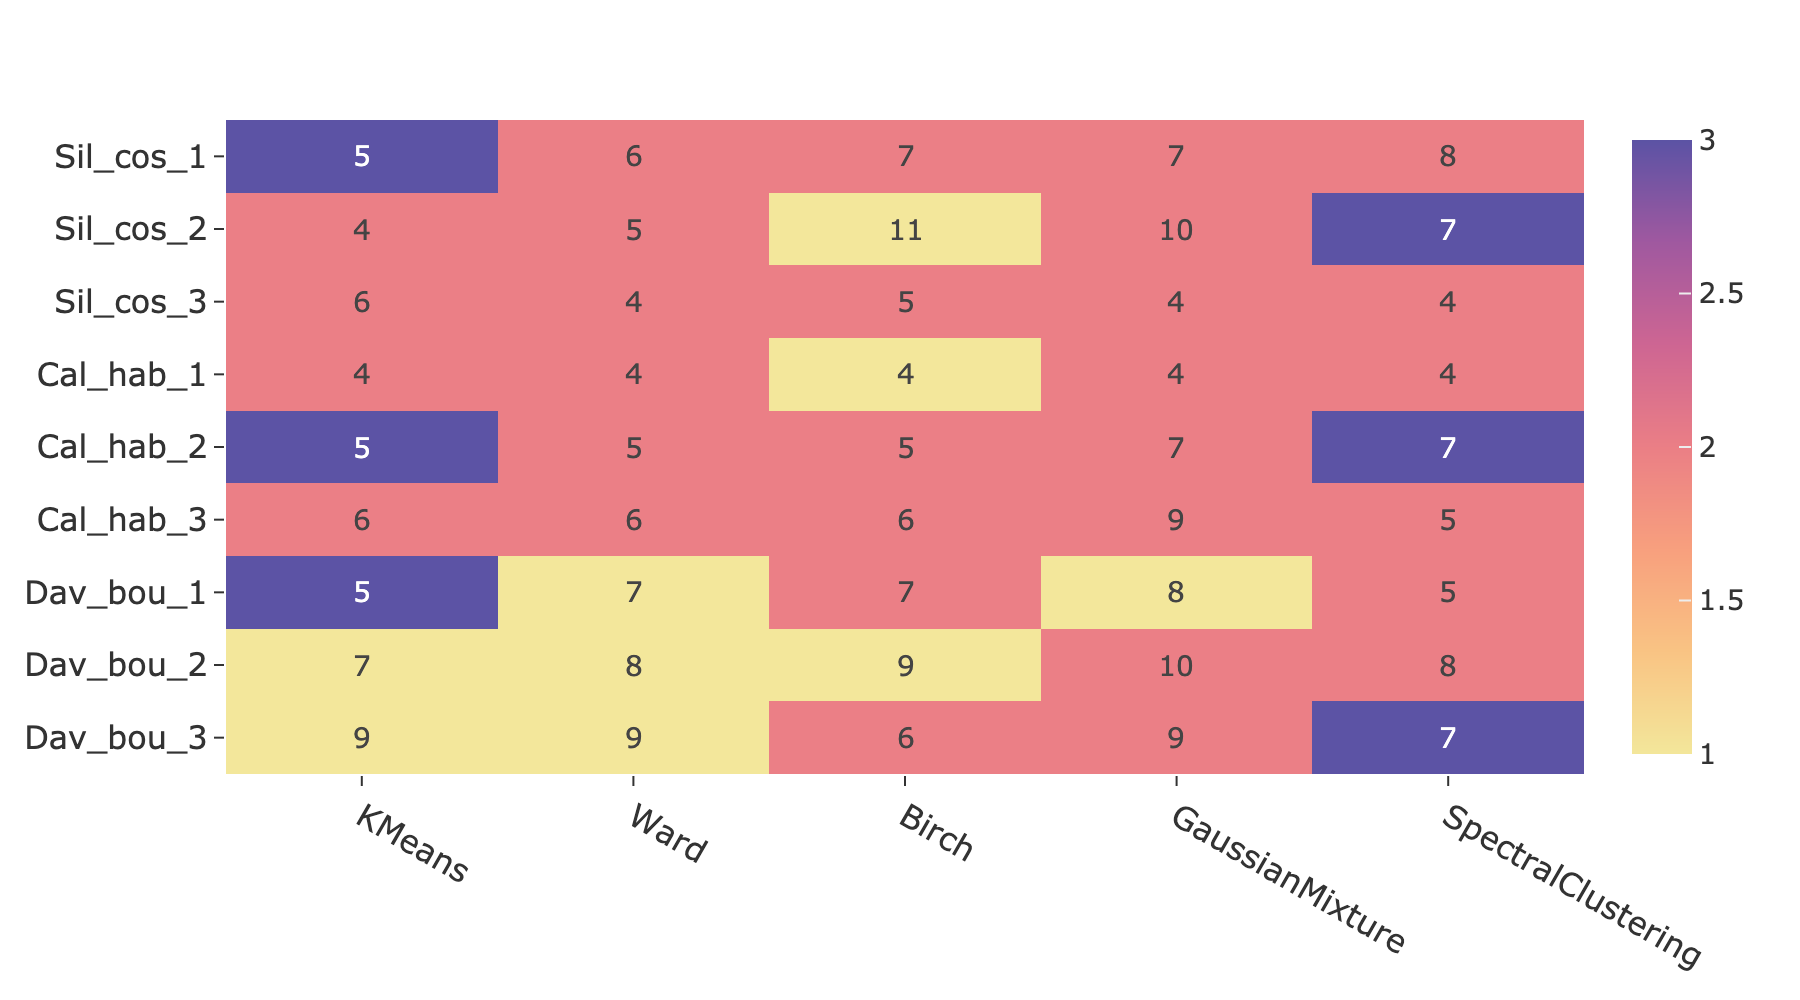
\includegraphics[width=\textwidth]{Sections/ClusteringAnalysis/Resources/cs_top3/top3_cs_size_top3_heatmap_pca.png}
        \caption{Most frequent cluster size}
        \label{fig:cs:heatmap_cs}
    \end{subfigure}
    \caption[Heatmaps: most common cluster model and $K$]{Most frequent model and K according to the clustering metrics. For each heatmap, the rows represent the top model/K for that metric, while the X-axis contains the methods used. The \textbf{colouring is per column}, allowing to determine of the optimal configuration per model and K. The following abbreviations were used: \textbf{Wrd} - Ward, \textbf{Brch} - Birch, \textbf{GaussianMixture} - Gaussian Mixture Models, \textbf{Spec} - Spectral Clustering. Both K-means with K=5 and Spectral Clustering with K=7 are the most frequent top scorers across the clustering models. Group sizes of 5 and 7 tend to score the highest across $K\in[3,13]$.}
    \label{fig:cs:cs_metrics_heatmap}
\end{figure}



\paragraph*{Silhouette distribution}

% Sillhouette
Hitherto, decision-making within this project has been guided by the average values derived from clustering metrics. While this approach informed the initial selection of the most suitable model, the K-means, and the optimal number of clusters, K=5, it inherently neglected the variability inherent in the scores. To address this analytical shortfall, the distribution of the Silhouette scores\footnote{This experiment is an adapted version of the \href{https://tinyurl.com/sillhouete-distrib}{example} provided by the Scikit-learn library.} are plotted in \cref{fig:cs:sill_distrib} for the K-means model, spanning 3 to 8 clusters. This restricted range was selected to improve visual interpretation and is supported by previous results (\cref{fig:cs:cs_metrics}), which indicate a decrease in cluster performance with higher K values, as was noticed before.


\begin{figure}[!t]
    \centering
    \captionsetup{font=small} 
    \begin{subfigure}[!t]{0.9\textwidth}
        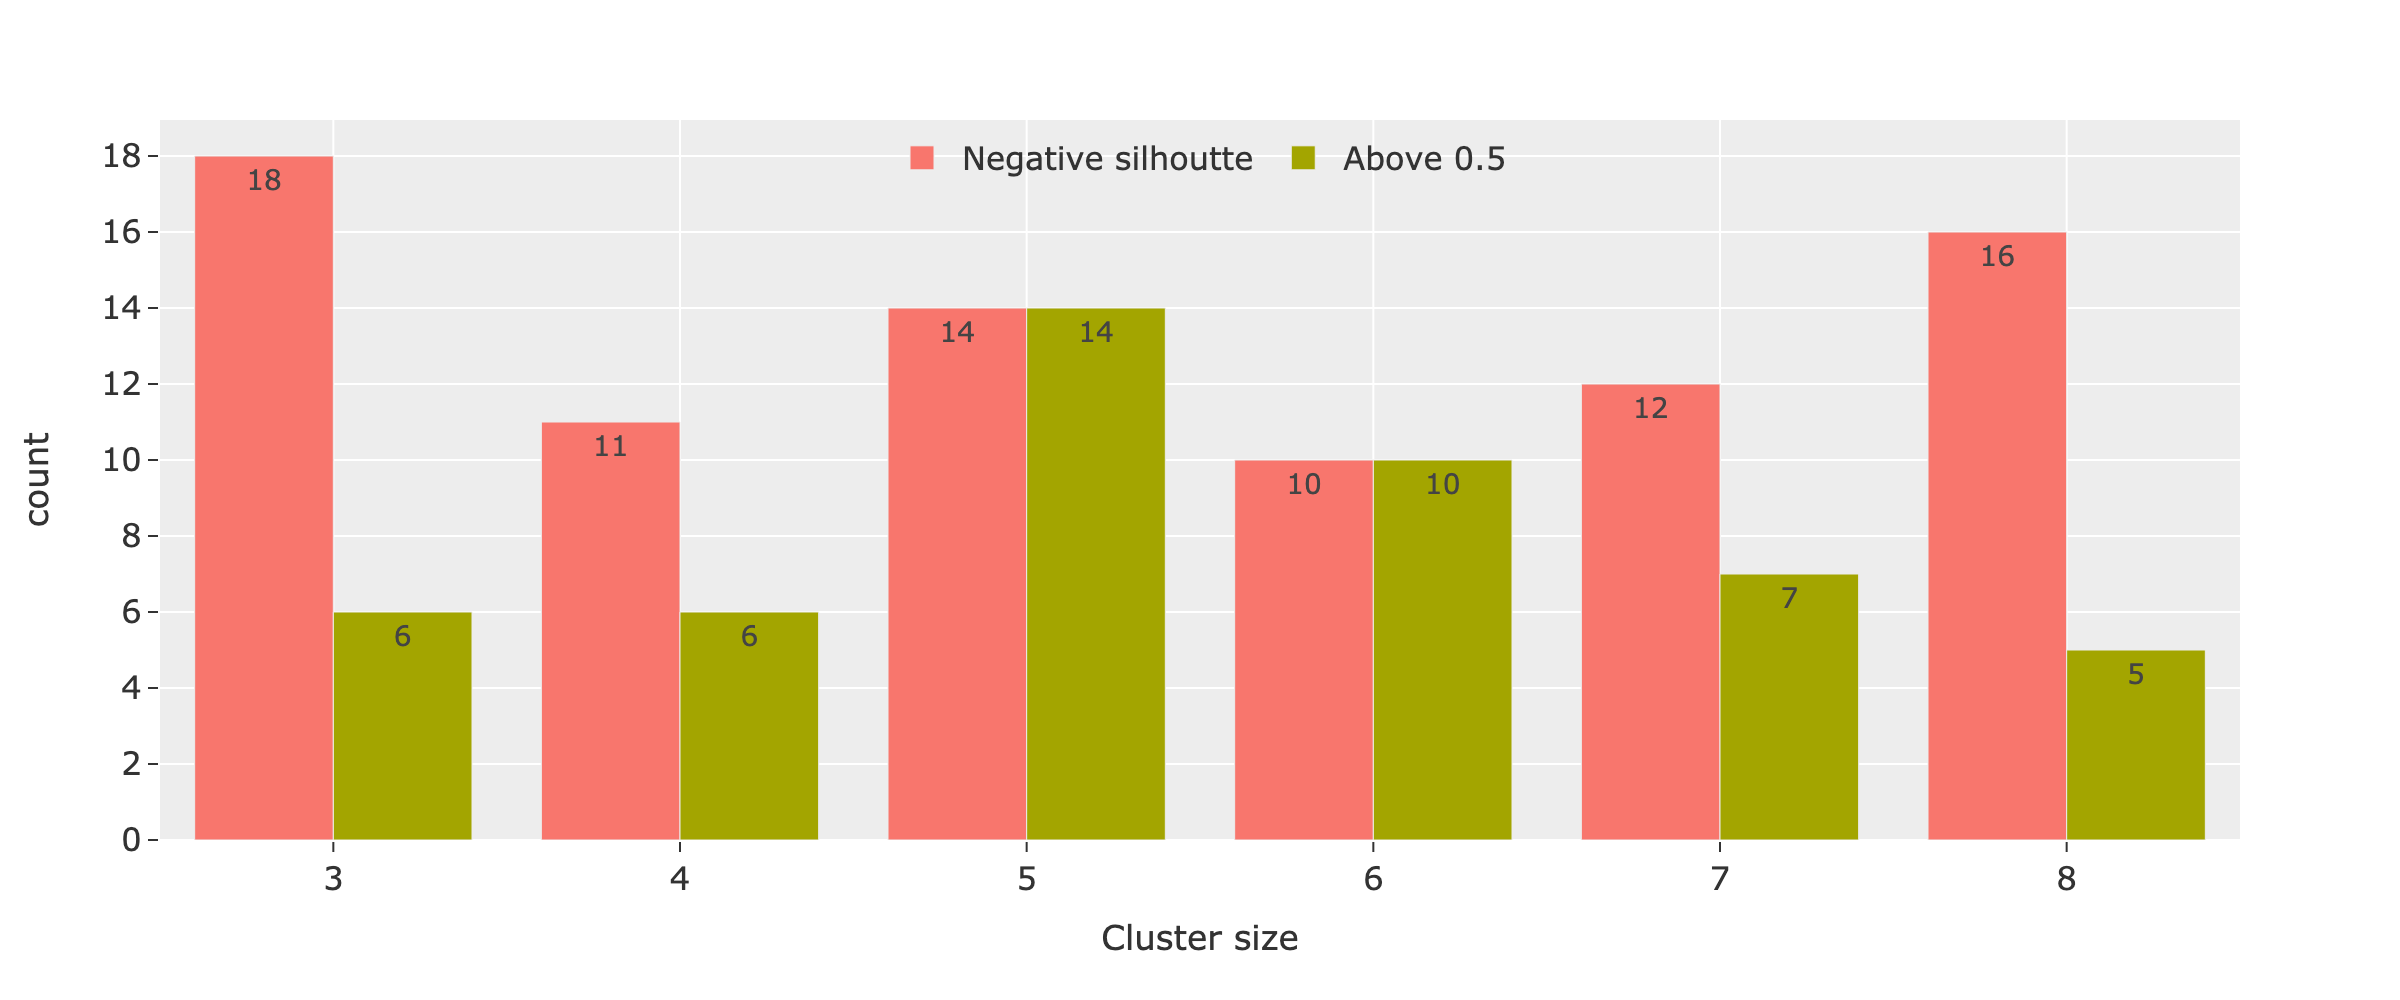
\includegraphics[width=\textwidth, keepaspectratio]{Sections/ClusteringAnalysis/Resources/cs_top3/sill_distrib/sill_neg_above_th.png}
        \caption{Number of samples with negative and above 0.5 Silhouette scores}
        \label{fig:cs:sill_neg_above_th}
    \end{subfigure}
    \centering
     \begin{subfigure}[!t]{0.9\textwidth}
        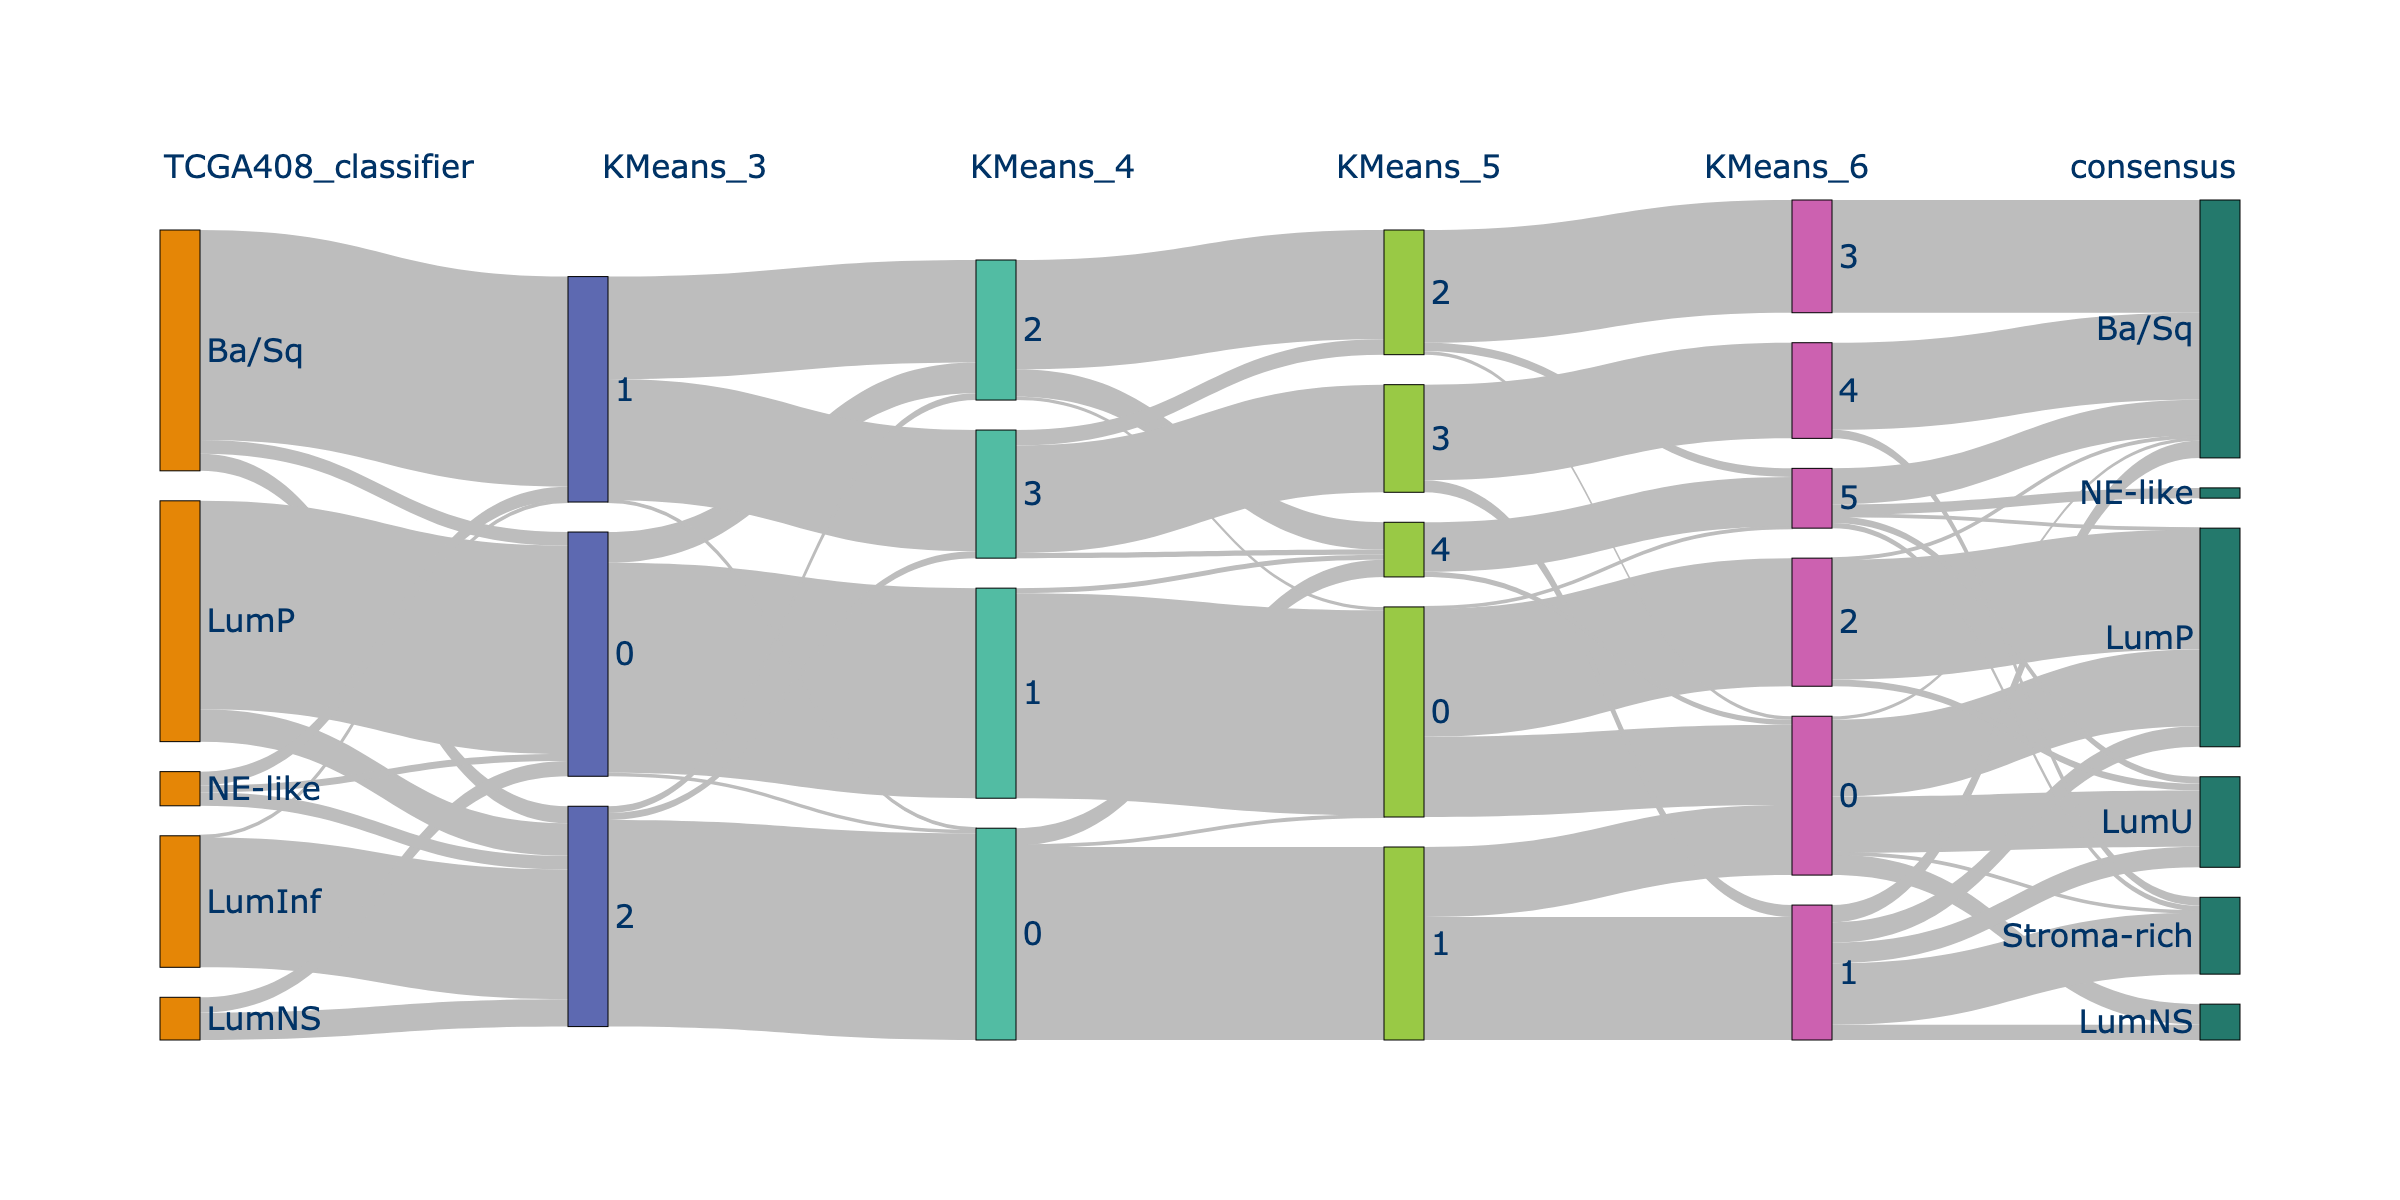
\includegraphics[width=\textwidth, keepaspectratio]{Sections/ClusteringAnalysis/Resources/cs_top3/sill_distrib/sky_kMeans.png}
        \caption{Comparison across clustering methods}
        \label{fig:cs:sankey_kMeans}
    \end{subfigure}
    \centering
    \caption[Mis-clustered samples overview]{The bar plot presents the number of samples with a Silhouette score above 0.5 (well-clustered) compared to those with negative values (poorly clustered). When the cluster size (K) is 5, there are the most well-clustered samples, while $K\in{3,8}$ has the most samples with negative values. The Sankey plot shows the comparison across the different configurations of K-Means. It can be seen that the Basal groups are split before the Luminal groups, which differs from other classifications in the literature \citep{Robertson2017-mg, Kamoun2020-tj}.}
    \label{fig:cs:sankey_comp}
\end{figure}


% Comment on the sillhouette distribution
The first two rows of \cref{fig:cs:sill_distrib} display subplots containing the Silhouette distribution and the 2-D scatter plot of the first two principal components. Across the top four plots, it is apparent that the vast majority of samples fall below the 0.5 threshold\footnote{In the research effort that introduced the Silhouette score \citep{Rousseeuw1987-wy}, the author indicates that positive values (closer to 1 are better) indicate well-separated groups, while negative values denote mis-clustering of the samples, and scores around 0 suggest that a sample could belong to multiple clusters. As a midpoint between 0 and 1, the Silhouette values $>$0.5 are considered to be well clustered.}, indicating a lack of clearly defined clusters and a high data heterogeneity, a known characteristic of the MIBC molecular profile; this was presented in more depth in \cref{s:lit:bladder_cancer}. Although K=3 has a higher mean score than other models, the top right plot shows that most samples still score below 0.5, as also confirmed in \cref{fig:cs:sill_neg_above_th}.


% Comment on the bar plot and the number of samples
The bar plot in \cref{fig:cs:sill_neg_above_th} displays the number of samples on the Y-axis for each $K \in [3, 8]$ that either exhibit negative Silhouette scores (red) or are above the 0.5 threshold (mustard). Across all $K$ values, there are few samples ($<$20) that exceed the recommended Silhouette threshold, indicating the lack of clearly defined groups. $K=5$ and $K=6$ show the highest number of well-clustered samples (14, 10), with $K=5$ also having an equal amount of samples with negative Silhouette scores. The highest instances of mis-clustered samples occur with $K=2$ and $K=3$, which also have the fewest samples (10) above the threshold. \Cref{fig:cs:sill_neg_above_th} suggests that the K-means with $K=5$ and $K=6$ perform better than the others by having the largest number of samples above the 0.5 threshold.


\begin{figure}[!t]
    \captionsetup[subfigure]{justification=Centering}
    \centering
    \begin{subfigure}[!t]{0.49\textwidth}
        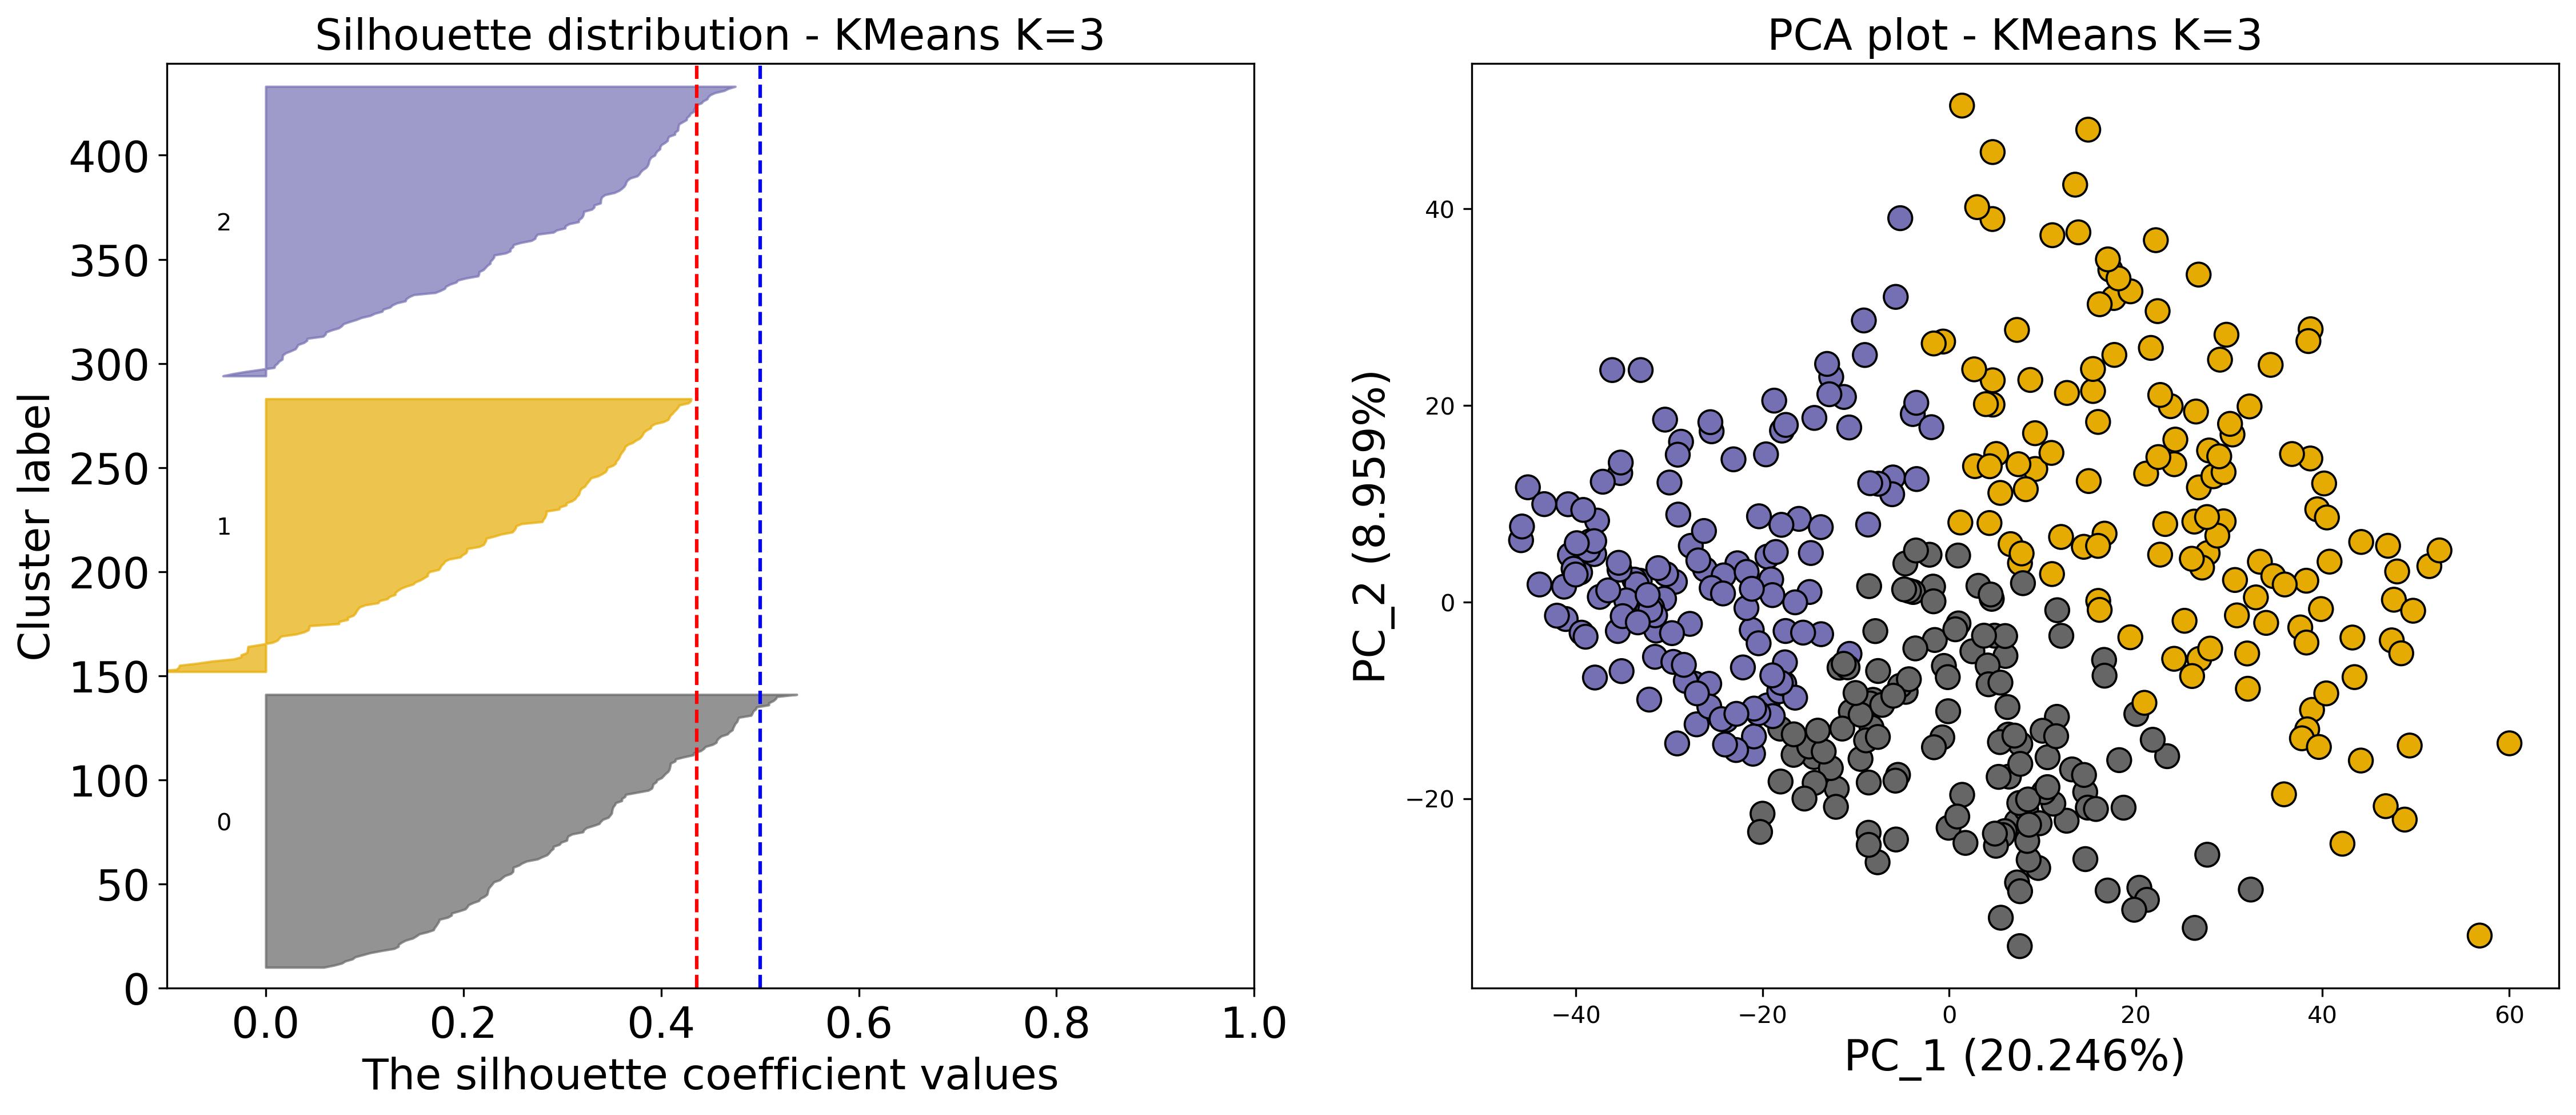
\includegraphics[width=\textwidth]{Sections/ClusteringAnalysis/Resources/cs_top3/sill_distrib/KMeans_3_sill_distrib.png}
        \caption{K=3 (Silhouette Mean: $0.43$)}
    \end{subfigure}
    \centering
    \begin{subfigure}[!t]{0.49\textwidth}
        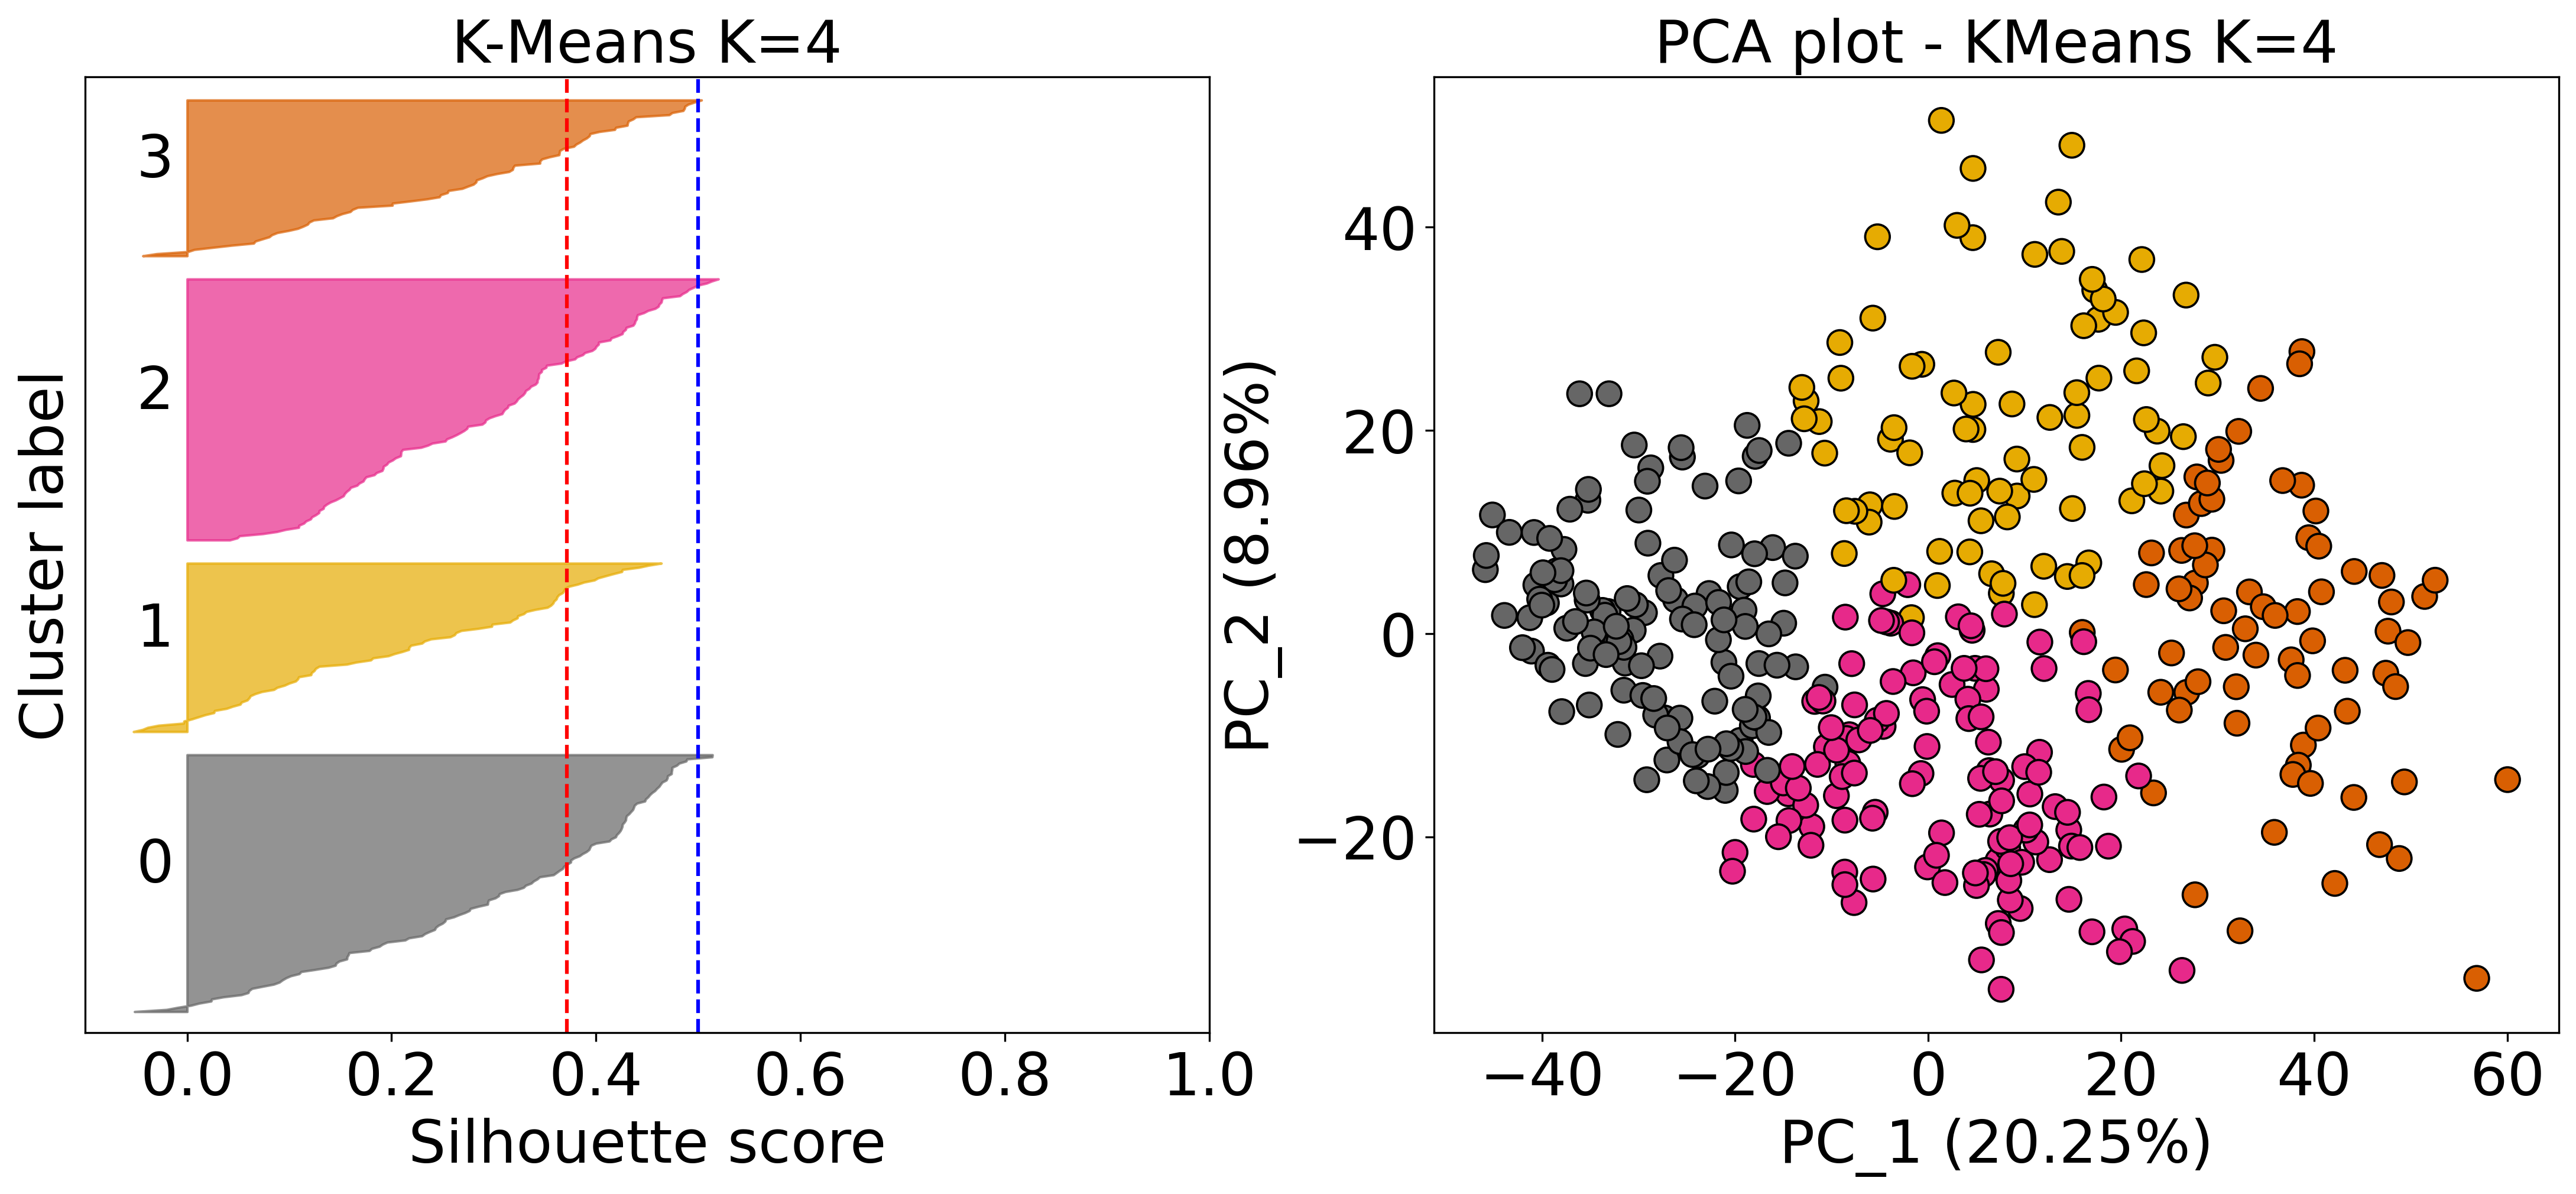
\includegraphics[width=\textwidth]{Sections/ClusteringAnalysis/Resources/cs_top3/sill_distrib/KMeans_4_sill_distrib.png}
        \caption{K=4 (Mean: $0.37$)}
    \end{subfigure}
    \centering
    \begin{subfigure}[!t]{0.49\textwidth}
        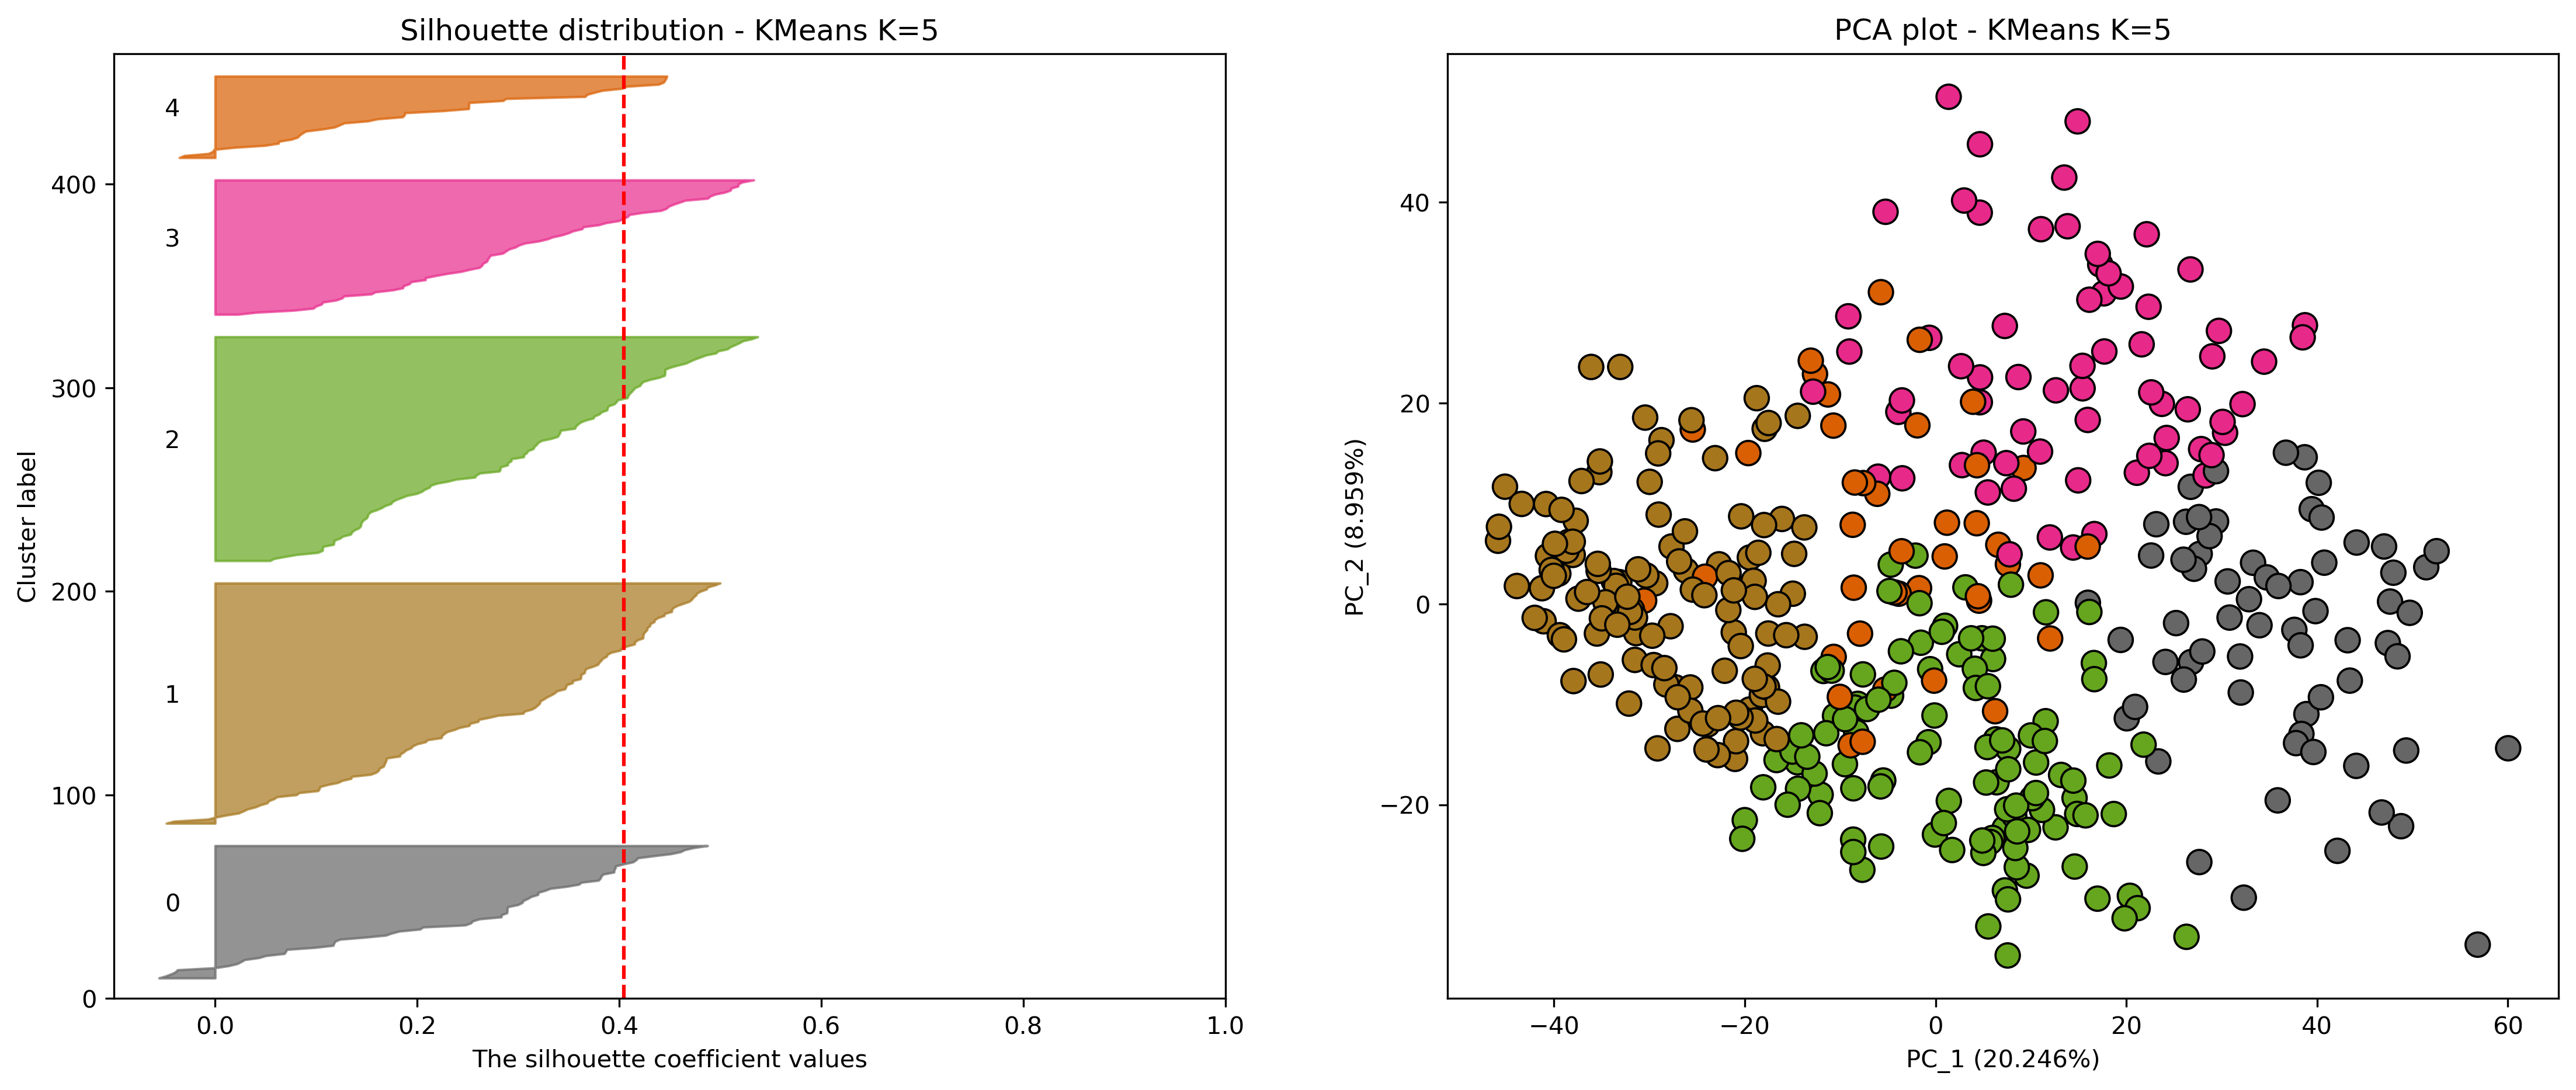
\includegraphics[width=\textwidth]{Sections/ClusteringAnalysis/Resources/cs_top3/sill_distrib/KMeans_5_sill_distrib.png}
        \caption{K=5 (Mean: $0.40$)}
    \end{subfigure}
    \centering
    \begin{subfigure}[!t]{0.49\textwidth}
        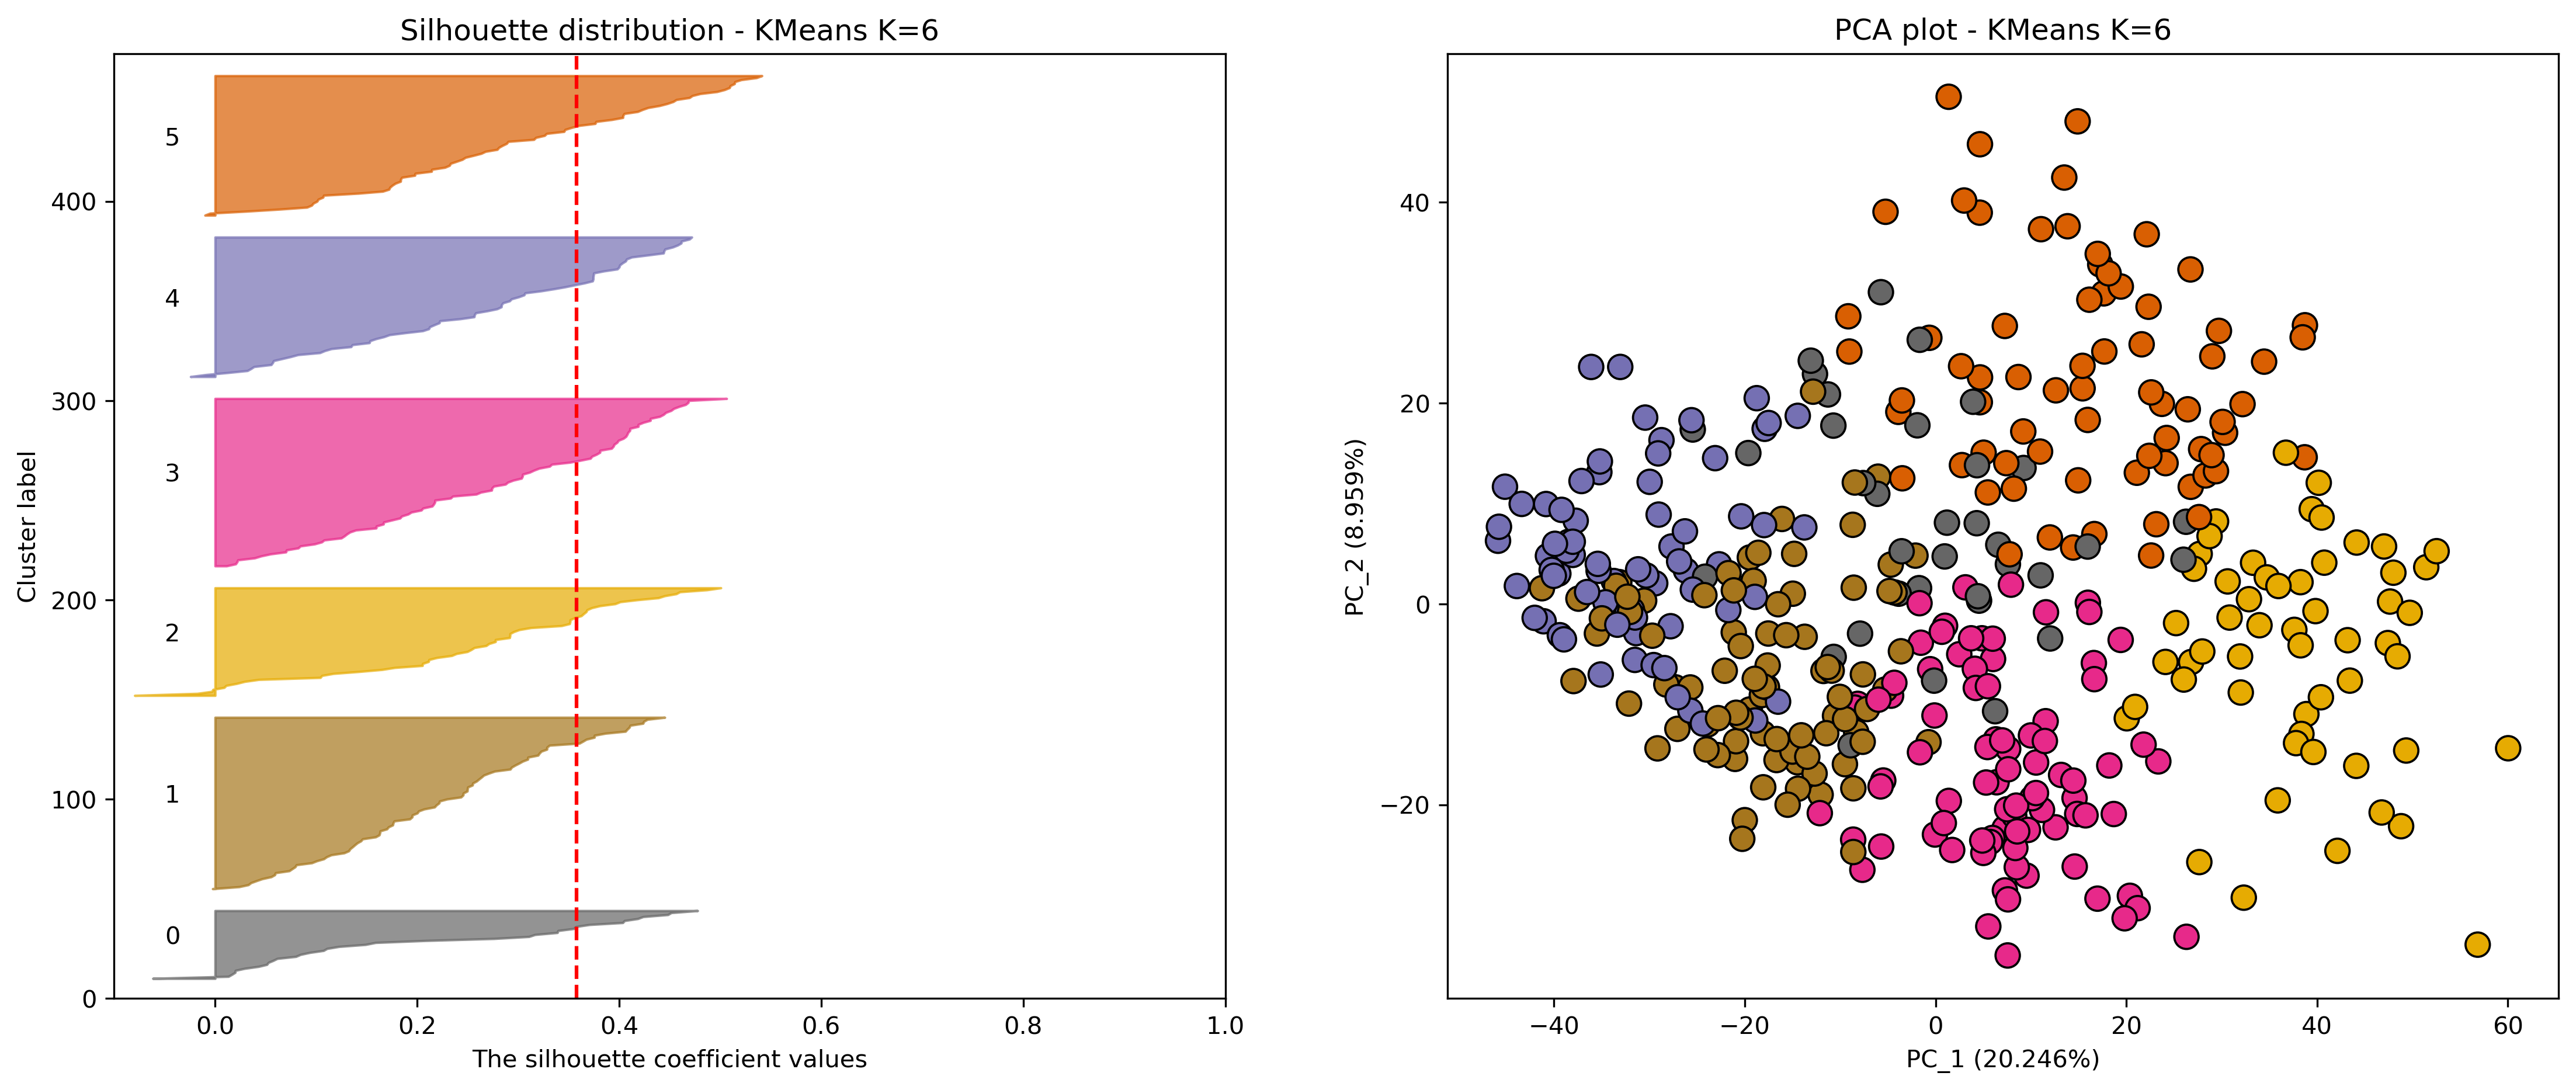
\includegraphics[width=\textwidth]{Sections/ClusteringAnalysis/Resources/cs_top3/sill_distrib/KMeans_6_sill_distrib.png}
        \caption{K=6 (Mean: $0.35$)}
    \end{subfigure}
    \centering
    \begin{subfigure}[!t]{0.49\textwidth}
        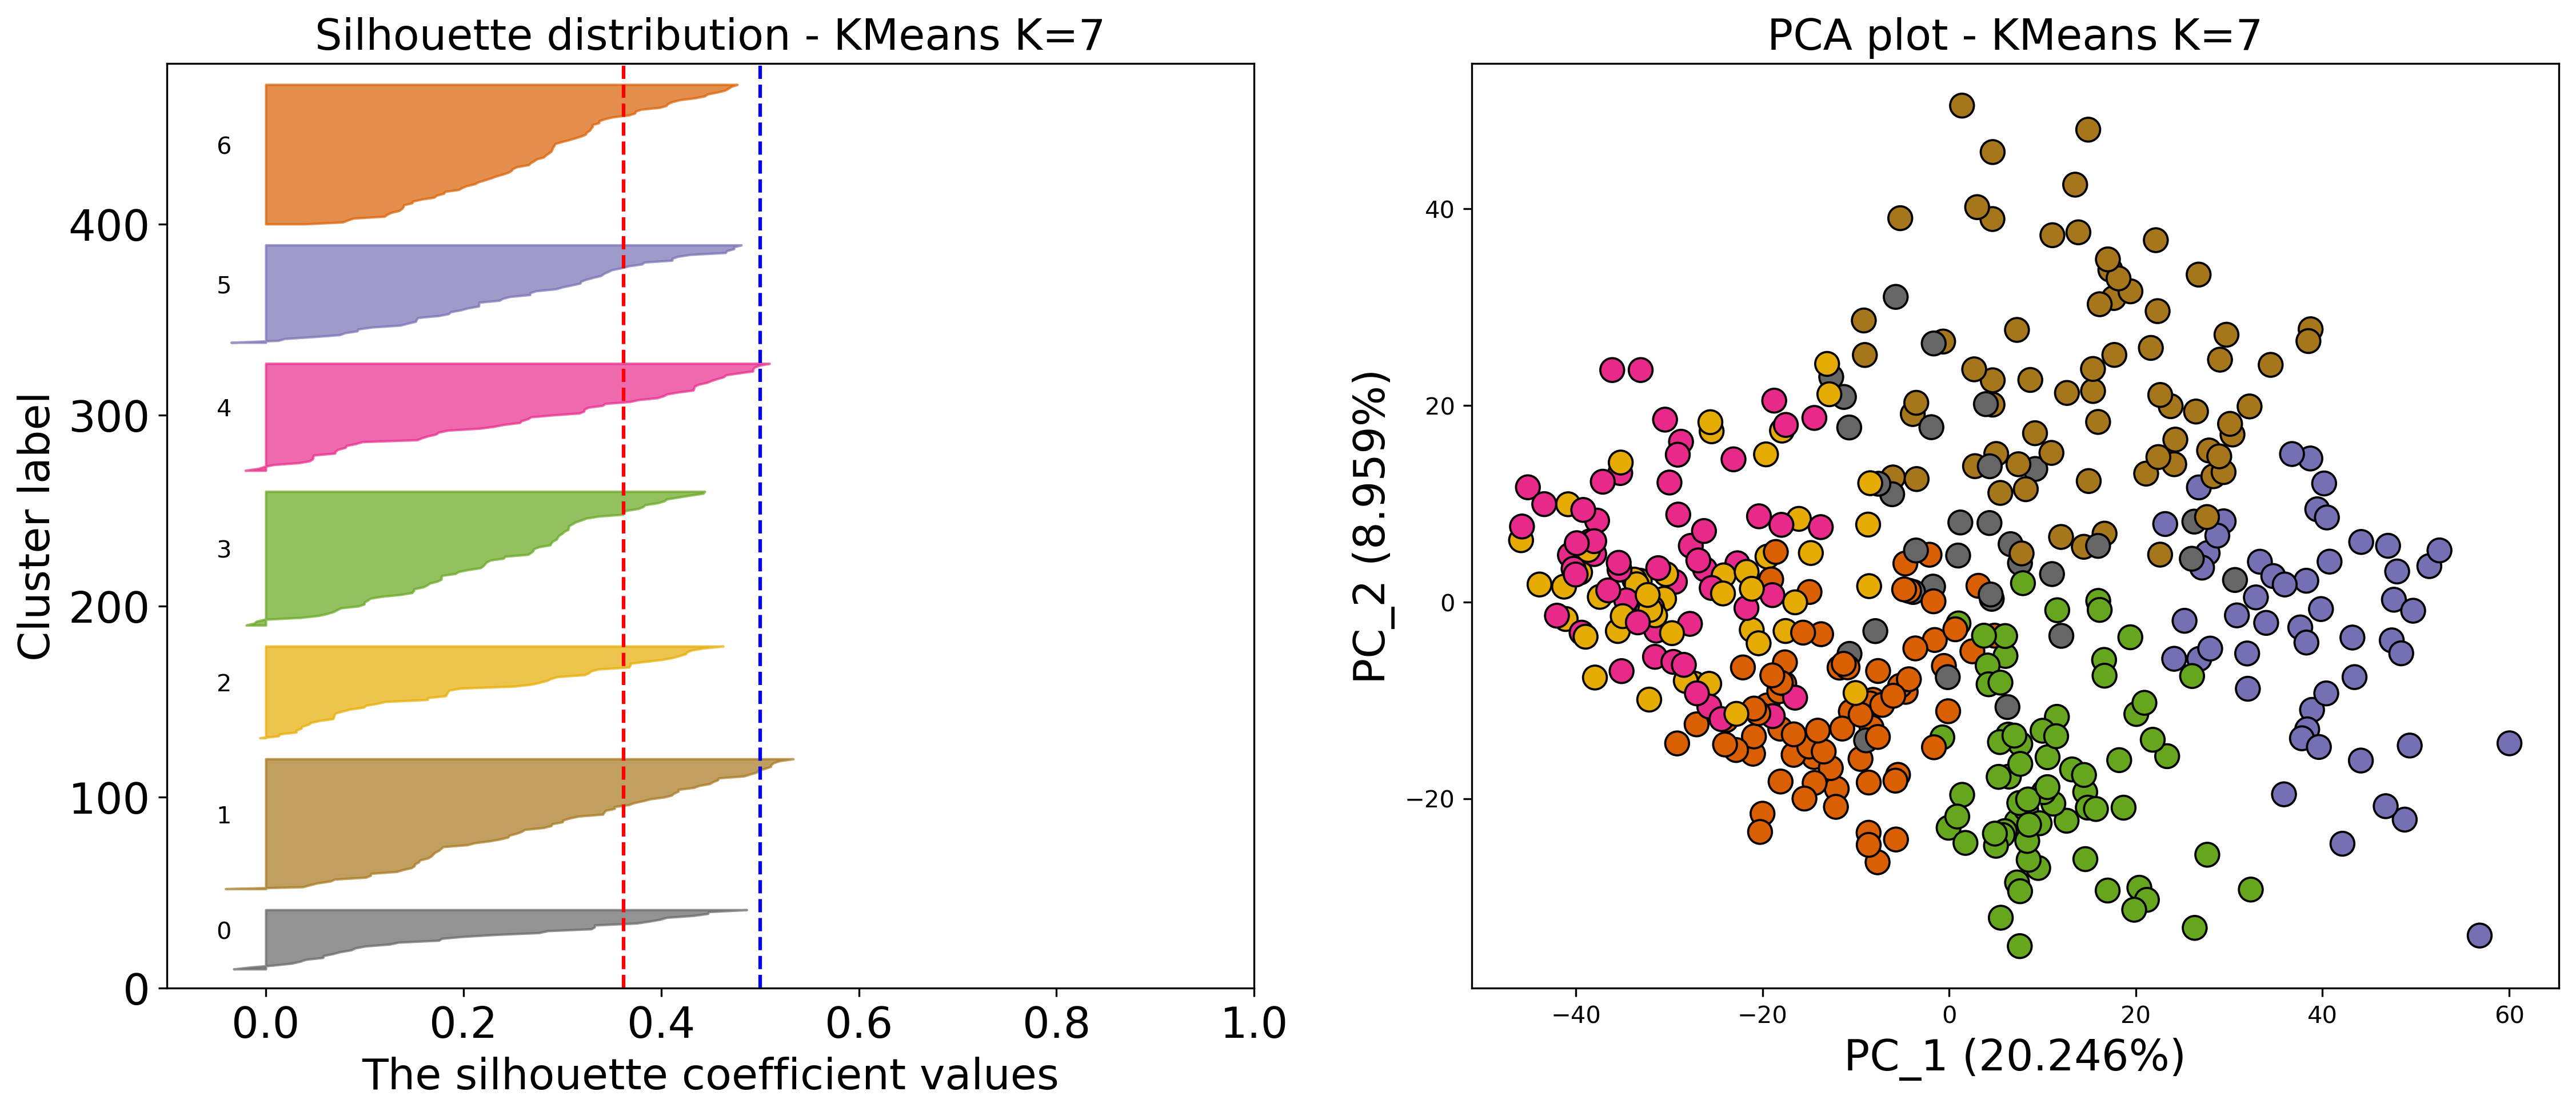
\includegraphics[width=\textwidth]{Sections/ClusteringAnalysis/Resources/cs_top3/sill_distrib/KMeans_7_sill_distrib.png}
        \caption{K=7 (Mean: $0.36$)}
    \end{subfigure}
    \centering
    \begin{subfigure}[!t]{0.49\textwidth}
        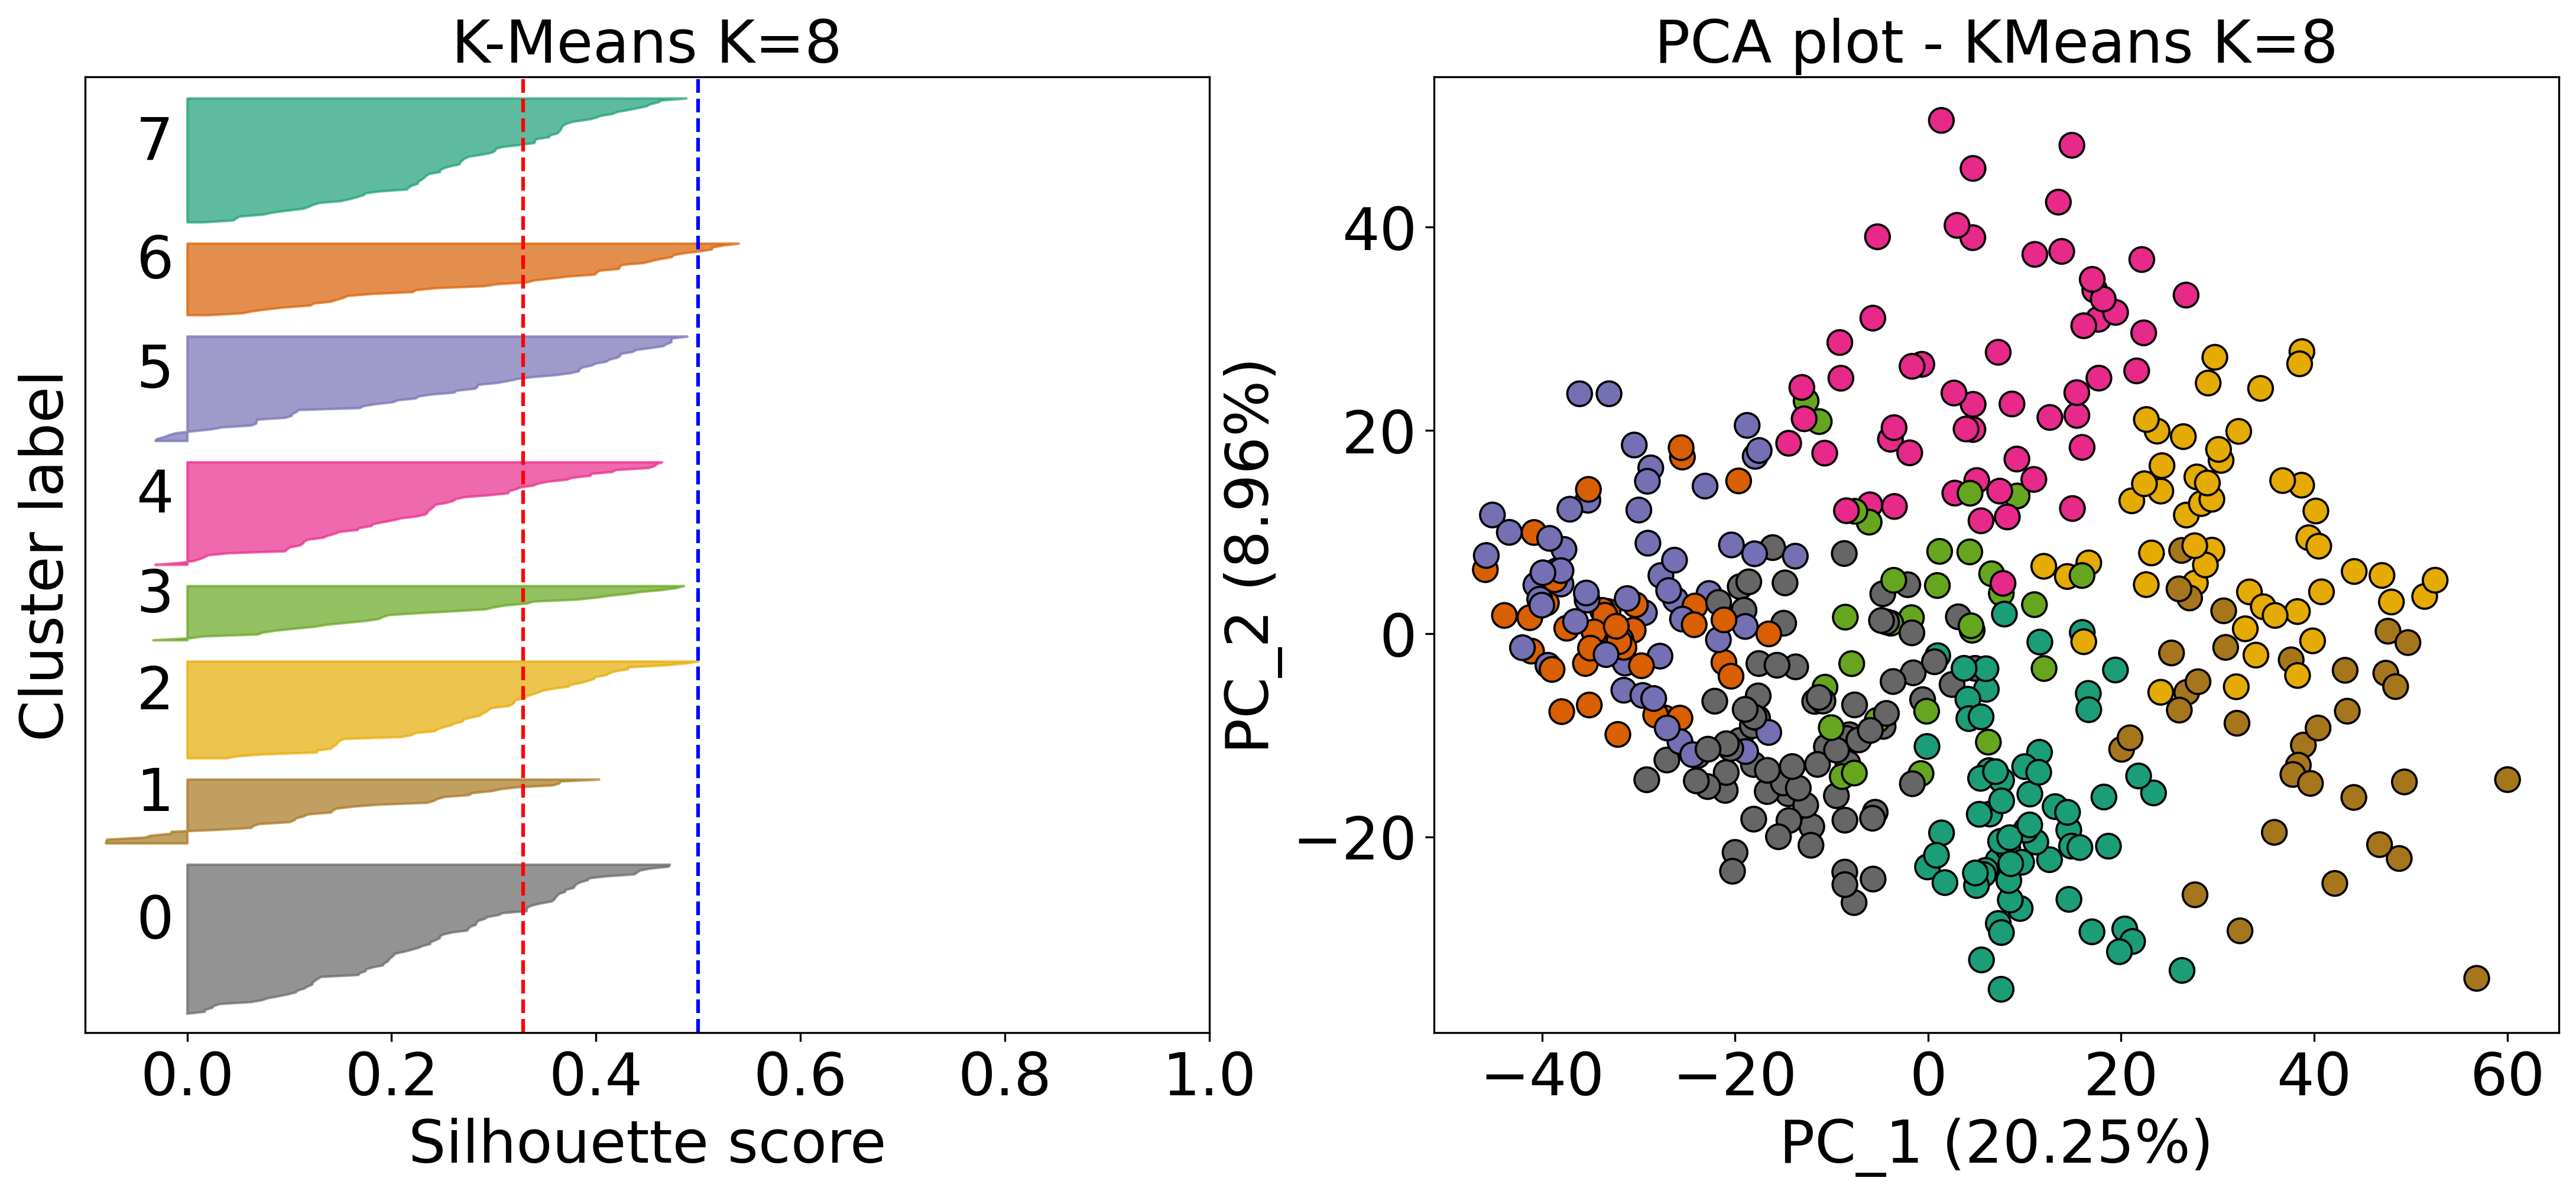
\includegraphics[width=\textwidth]{Sections/ClusteringAnalysis/Resources/cs_top3/sill_distrib/KMeans_8_sill_distrib.png}
        \caption{K=8 (Mean: $0.32$)}
    \end{subfigure}
    \centering
    \caption[Silhouette distribution a further exploration of K-means]{The Silhouette distribution of the K-means model for K ranging from 3 to 8. The scatter plot on the right displays the first 2 components of PCA (out of 4 components) coloured by the cluster labels from the method. A good Silhouette score is considered to be above 0.5, which is marked by the blue dotted line. The red dotted line represents the mean value. The values in the brackets represent the mean Silhouette scores across the samples. The figures provide a complete picture of the Silhouette scores for different K-values, including the proportion of negative values (indicating poor clustering) and their representation in the first two Principal Components. The highest mean Silhouette score is achieved when K=3, followed by K=5 and K=4. The number of negative Silhouette samples for each K is shown in \cref{fig:cs:sill_neg_above_th}.}
    \label{fig:cs:sill_distrib}
\end{figure}

Lastly, the Sankey plot visualises the cluster evolution as $K$ increases. Initially, at $K=3$, three groups are identified: Basal, Luminal, and Luminal Infiltrated. As $K$ increases to 4, the Basal group divides into four subgroups, which then consolidate into three at $K=5$; these subgroups are maintained through $K=6$. Surprisingly, the large Luminal group only splits at $K=6$, which deviates from previous TCGA classifications or consensus \citep{Robertson2017-mg, Kamoun2020-tj} where the Luminal group typically divides into smaller subgroups earlier than the Basal.

Based on the analysis conducted in this section, $K=5$ and $K=6$ emerge as the most suitable configurations for the model. Specifically, $K=5$ consistently ranks among the three best performing models, as evidenced in \cref{fig:cs:cs_metrics} and \cref{fig:cs:cs_metrics_heatmap}. Given the clustering metrics, $K=5$ was selected over $K=6$ as the configuration moving forward.





% pipeline
\subsection{Pipeline}

The pipeline and configuration of the different components can be summarised in \cref{fig:cs:clustering_pipeline} and has three stages:
\begin{enumerate}
    \item \textbf{Data pre-processing} - only the genes that are expressed in 90\% of the samples are selected, resulting in a dataset of $\sim$15000 genes
    \item \textbf{Gene selection} - the top $3500$ with the highest std/median ratio are kept. The number of genes represent $\sim$25\% of the filtered dataset and it is a similar size to the data used by \citet{Robertson2017-mg}
    \item \textbf{Dimension reduction} - of the resultant gene set of 408 samples by 3500 genes is $log2(TPM+1)$ transformed and the PCA with 4 components is applied
    \item \textbf{Clustering} - on the 408 samples by 4 Principal Components (PCs) the K-mean clustering algorithm with $K=5$ is applied, resulting in five groups displayed in the first two principal components at the end of the pipeline
\end{enumerate}

% Interpreting the Sankey plot
The cluster analysis established in this part of the thesis uses computational methods without domain knowledge to arrive at the configuration of K means with K = 5. It can be seen that the number of clusters that arrive is the same as in the TCGA classifier \citep{Robertson2017-mg} and that consensus found 6 subtypes \citep{Kamoun2020-tj}. The developed clustering method is used at the different stages of the project to determine the clustering configuration \cref{s:ap:p0_clustering,s:ap:N_II:clustering analysis}.

% Introducing the next chapter
Next in the chapter, the five clusters are explored in more depth and put in the context of \textit{in vitro} work performed in the Jack Birch Unit by \citet{Baker2022-bj}, TCGA, Lund and the consensus classifiers \citep{Robertson2017-mg, Marzouka2018-ge, Kamoun2020-tj}. It will also cover their clinical implication by performing Kaplan-Meier survival analysis and \acrlong{dea}.

% Implementation details
\subsection*{Implementation details}

The following adjustments based on \citet{Scikit-learn_undated-ax} were made to the default settings of the models to optimise the clustering outcomes:
\begin{itemize}
    \item \textbf{K-Means:} Maximum iterations increased to 1000.
    \item \textbf{Ward:} Employed agglomerative clustering with Ward linkage and a connectivity matrix computed using 5 nearest neighbours for each point.
    \item \textbf{Birch:} The threshold parameter `birch\_th` was set to 1.7
    \item \textbf{Gaussian Mixture:} The covariance type was set to diagonal with maximum iterations capped at 500.
    \item \textbf{Spectral Clustering:} Eigenvalue decomposition was performed using arpack and the affinity matrix was based on nearest neighbours.
\end{itemize}

